\subsubsection{External Interface Requirements}
This section of the document gives a clear description of all the requirments that the system needs in order to performe all 
the functionalities described in section \ref{subsection:2.2}.

\subsubsection{User Interfaces}
The following mockups of the web application provide a first idea on how the features of the system are offered to the users. 
Moreover it gives a real perpespective of how the users interact with the system. 
The Design Document (reference) provides a thorough and detailed description of the features represented in each mockup.

\begin{figure}[H]
    \begin{center}
    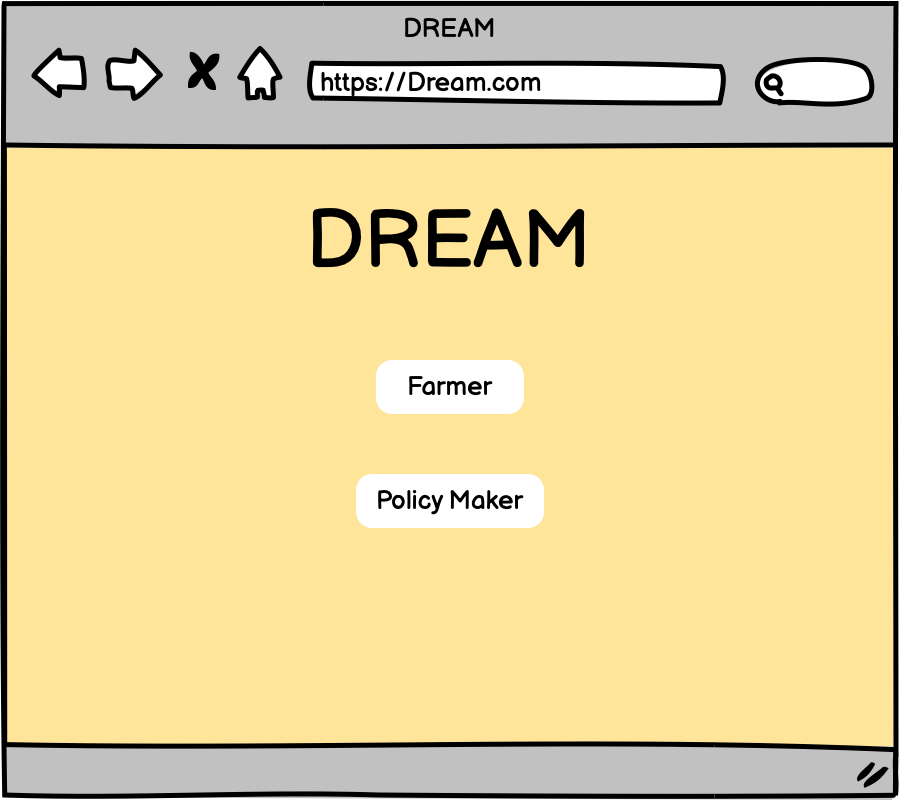
\includegraphics[width=0.6\textwidth]{mockups/Dream.png}
    \caption{\emph{DREAM} Web page}
    \label{fig:webPage}
    \end{center}
\end{figure}
 
\begin{figure}[ht!]
    \begin{minipage}{0.5\textwidth}
        \centering
        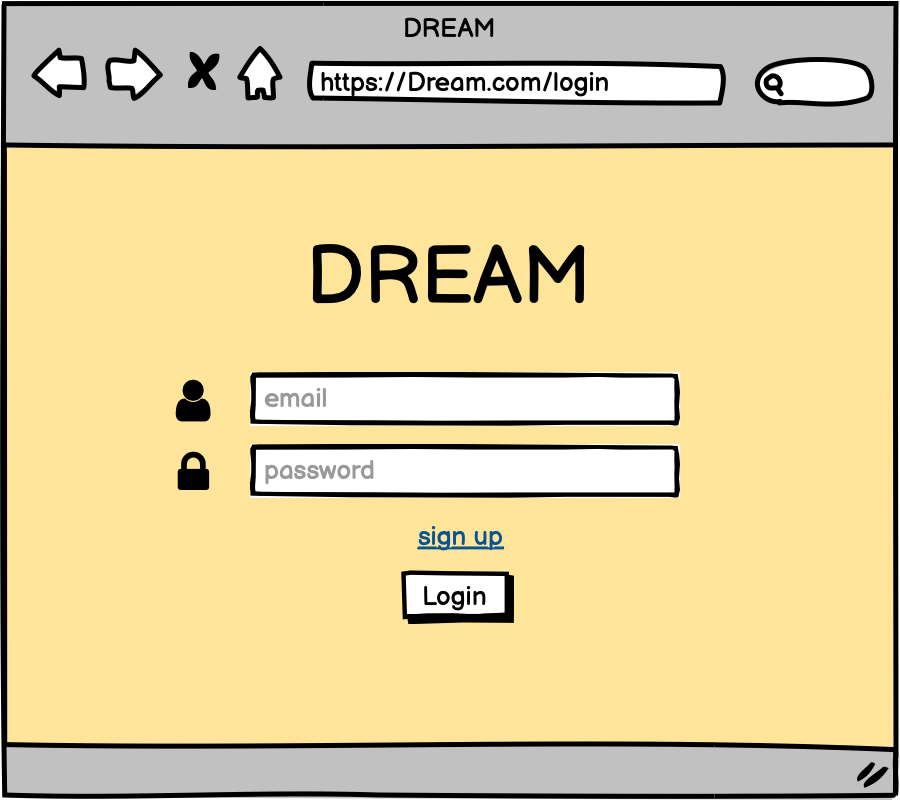
\includegraphics[width=1\textwidth]{mockups/FLogIn.png}
        \caption{\emph{Farmer Log in} Web page}
        \label{fig:mockupLogin}
    \end{minipage}\hfill
    \begin{minipage}{0.5\textwidth}
        \centering
        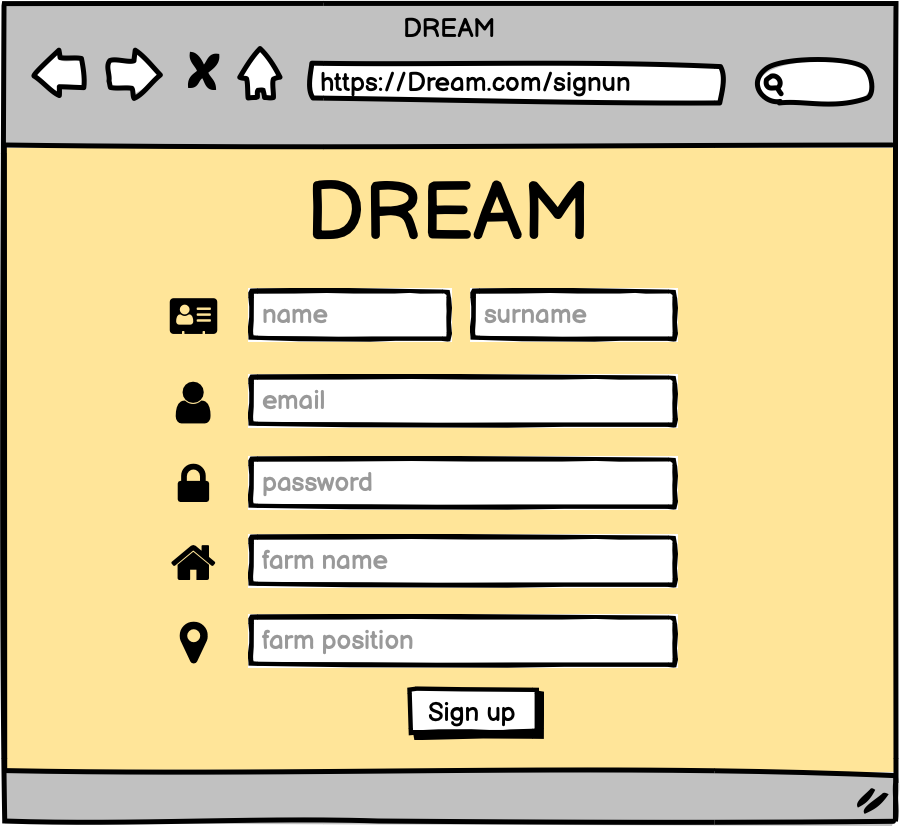
\includegraphics[width=1\textwidth]{mockups/SignUp.png}
        \caption{\emph{Farmer Sign up} Web page}
        \label{fig:smockupSignUp}
    \end{minipage}
\end{figure}

\begin{figure}[H]
    \begin{center}
    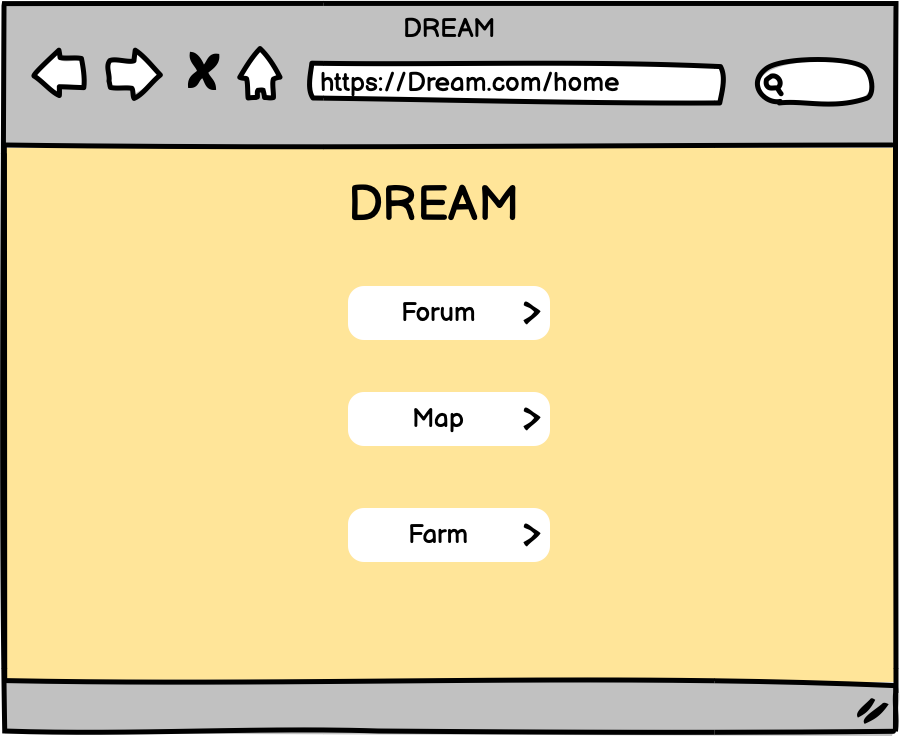
\includegraphics[width=0.6\textwidth]{mockups/FHome.png}
    \caption{\emph{Farmer} Home page}
    \label{fig:homepage}
    \end{center}
\end{figure}

\begin{figure}[H]
    \begin{center}
    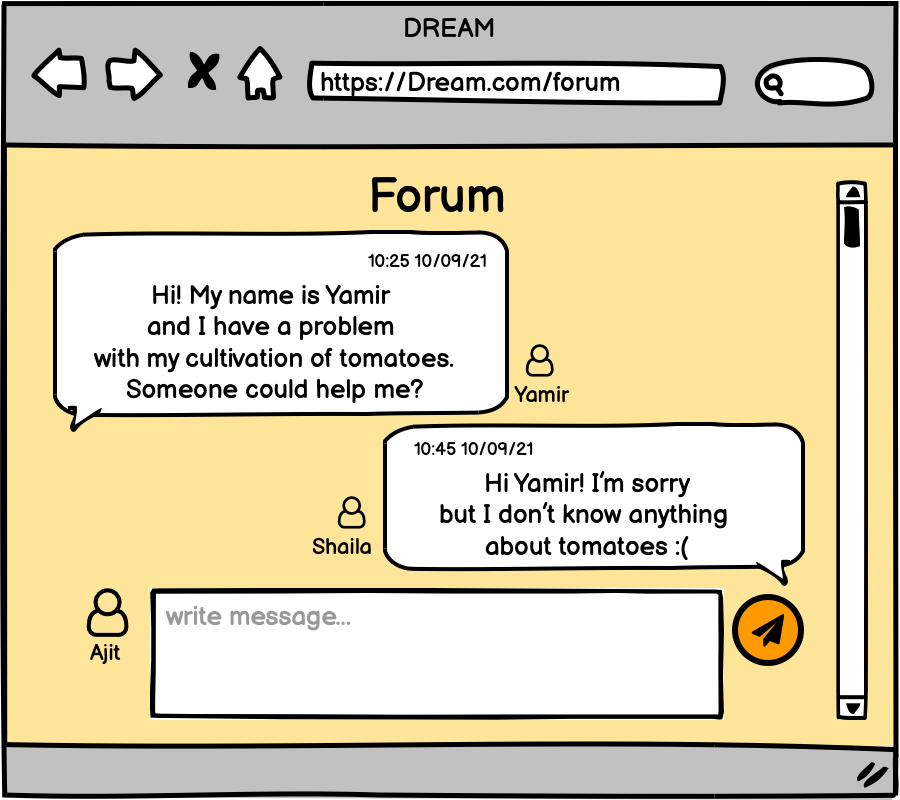
\includegraphics[width=0.7\textwidth]{mockups/Forum.png}
    \caption{\emph{Forum} Web page}
    \label{fig:forum}
    \end{center}
\end{figure}

\begin{figure}[H]
    \begin{center}
    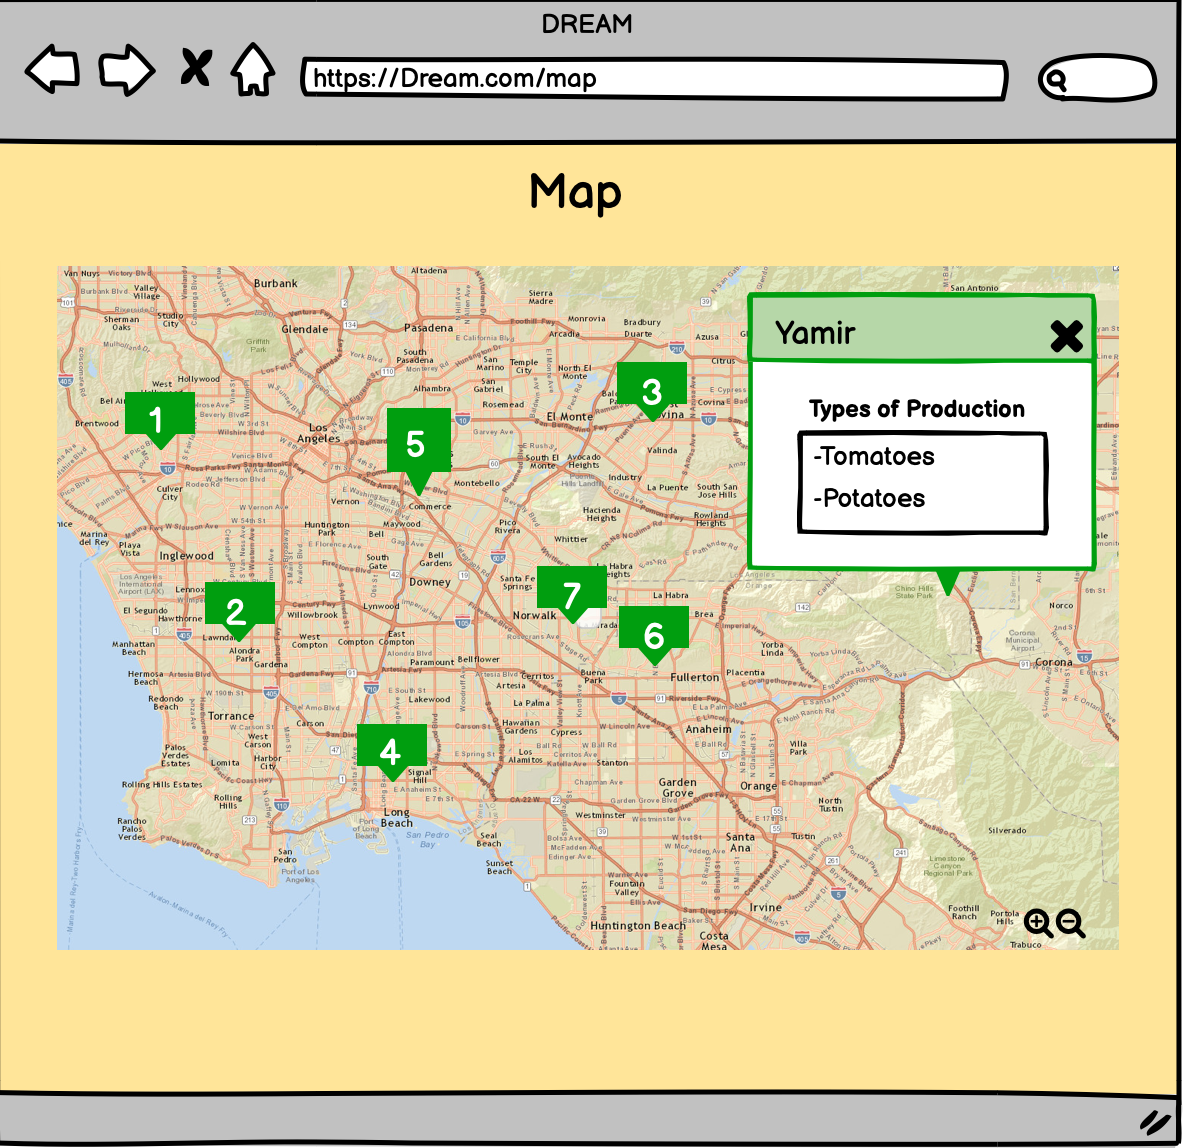
\includegraphics[width=0.7\textwidth]{mockups/FMap.png}
    \caption{\emph{Farmer } Map page}
    \label{fig:farmerMap}
    \end{center}
\end{figure}

\begin{figure}[H]
    \begin{center}
    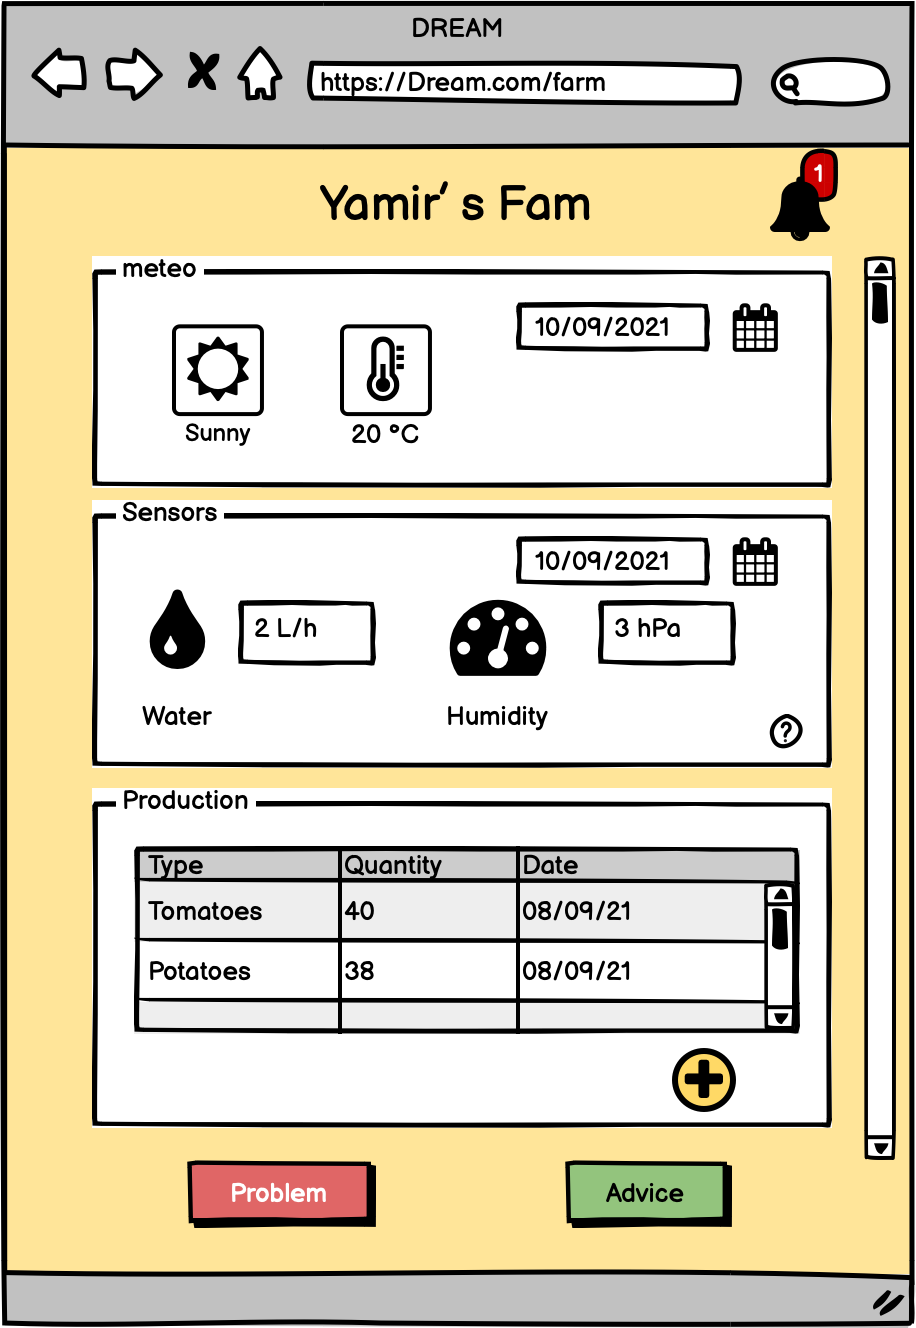
\includegraphics[width=0.7\textwidth]{mockups/FFarm.png}
    \caption{\emph{Farmer's} Farm page}
    \label{fig:FarmPage}
    \end{center}
\end{figure}

\begin{figure}[H]
    \begin{center}
    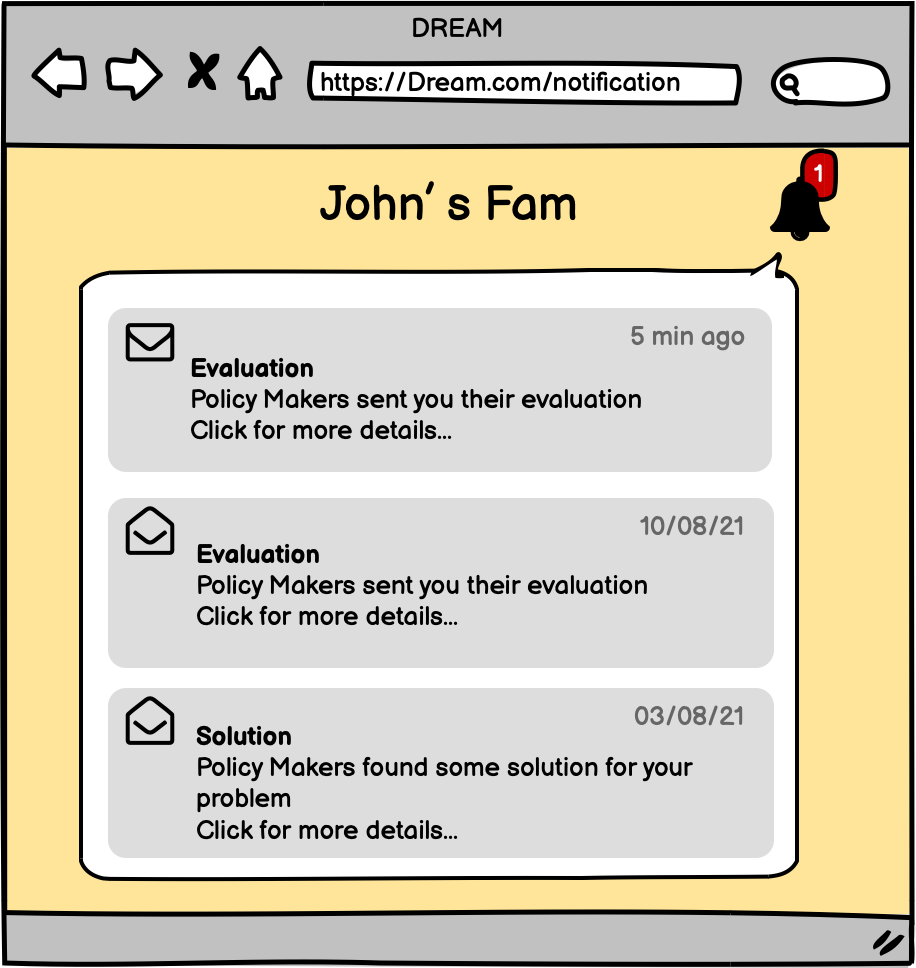
\includegraphics[width=0.7\textwidth]{mockups/Notifications.png}
    \caption{\emph{Farmer's notifications list}}
    \label{fig:notificationList}
    \end{center}
\end{figure}

\begin{figure}[H]
    \begin{center}
    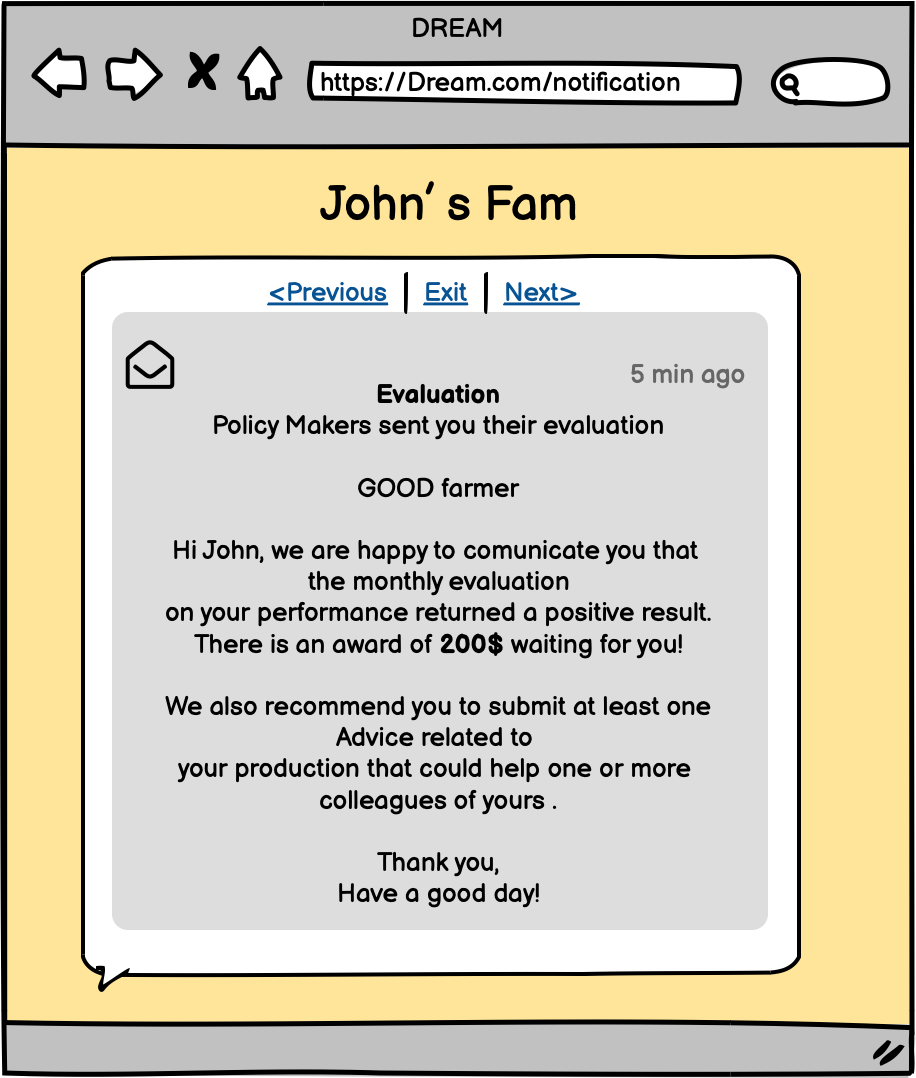
\includegraphics[width=0.7\textwidth]{mockups/Notification.png}
    \caption{\emph{Farmer's single notification}}
    \label{fig:singleNotification}
    \end{center}
\end{figure}

\begin{figure}[H]
    \begin{center}
    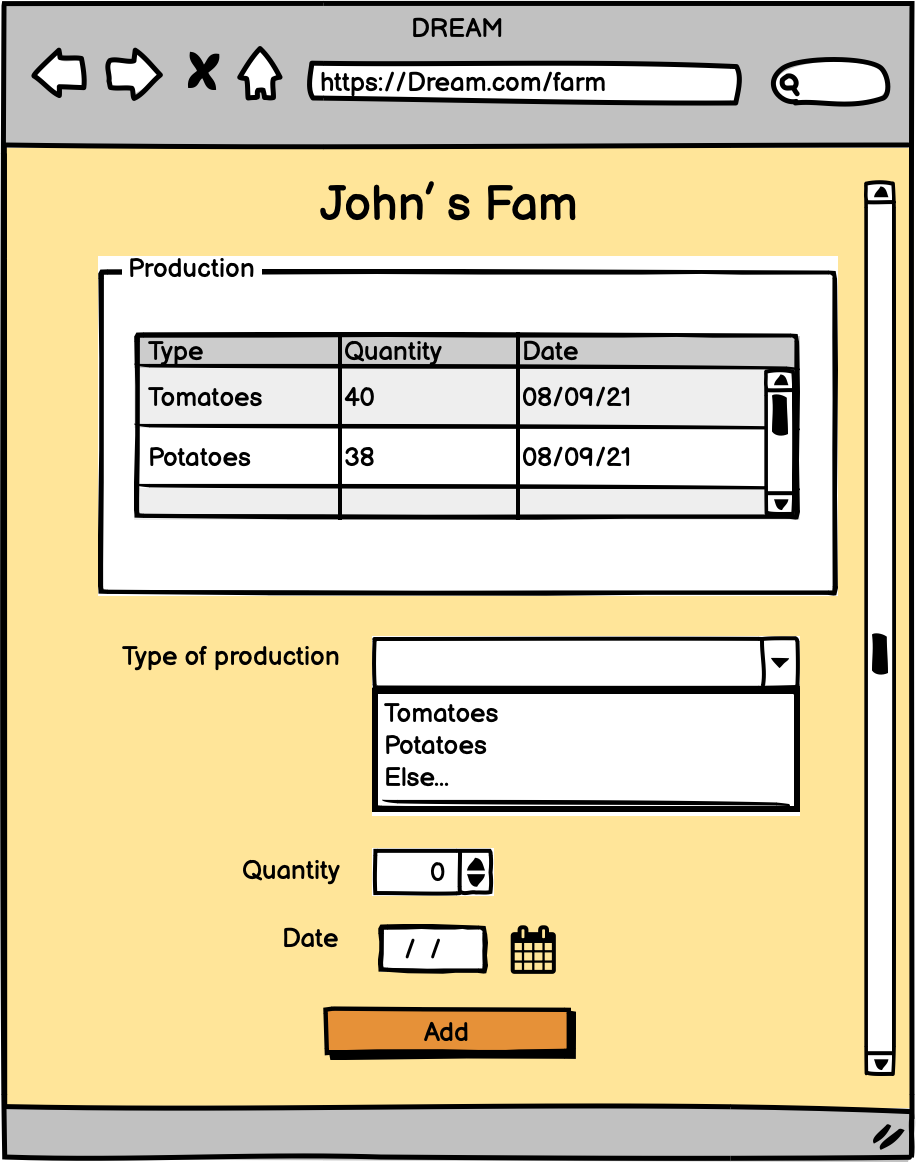
\includegraphics[width=0.7\textwidth]{mockups/AddData.png}
    \caption{\emph{Farmer add data} Web page}
    \label{fig:addData}
    \end{center}
\end{figure}

\begin{figure}[H]
    \begin{center}
    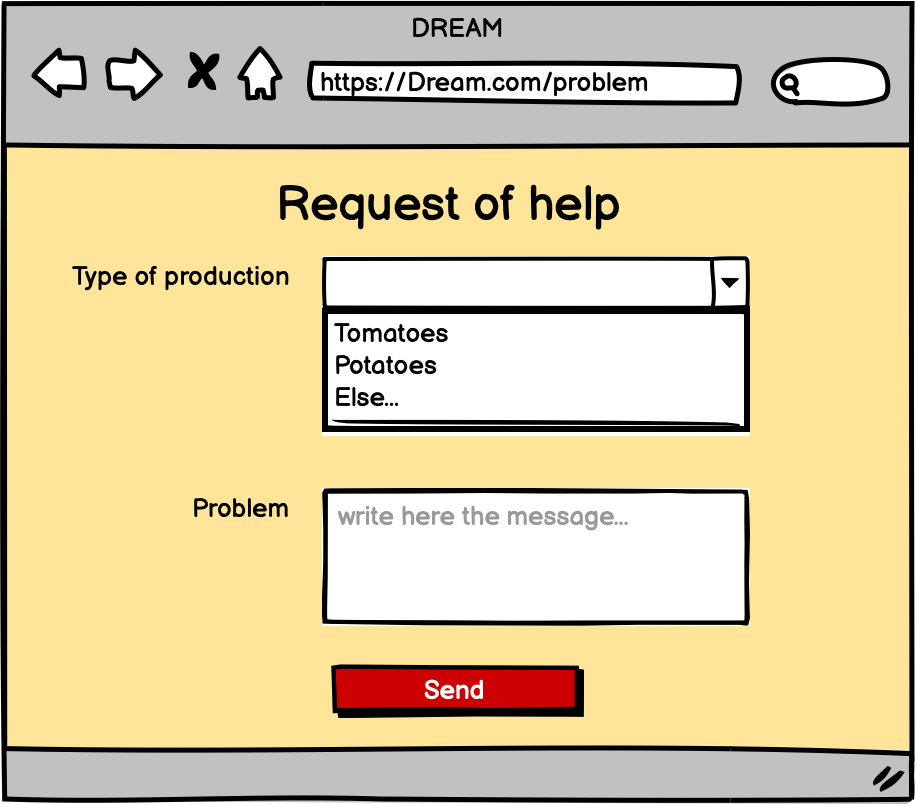
\includegraphics[width=0.7\textwidth]{mockups/Help.png}
    \caption{\emph{Farmer send request of help} Web page}
    \label{fig:helpRequest}
    \end{center}
\end{figure}

\begin{figure}[H]
    \begin{center}
    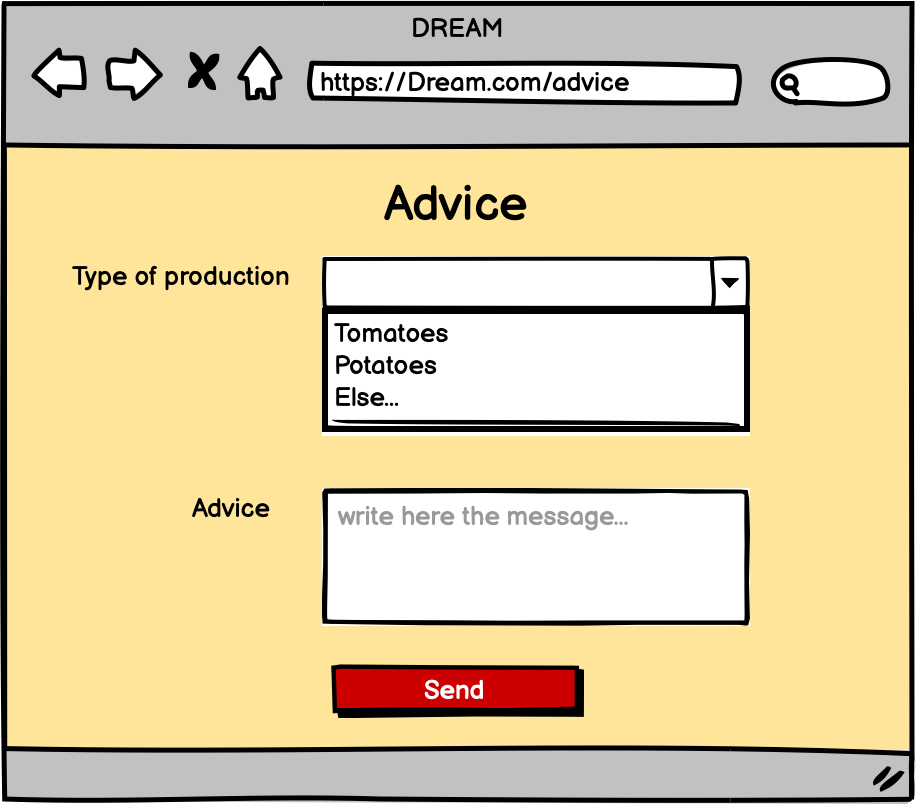
\includegraphics[width=0.7\textwidth]{mockups/Advice.png}
    \caption{\emph{Farmer submit advice} Web page}
    \label{fig:submit advice}
    \end{center}
\end{figure}

\begin{figure}[H]
    \begin{center}
    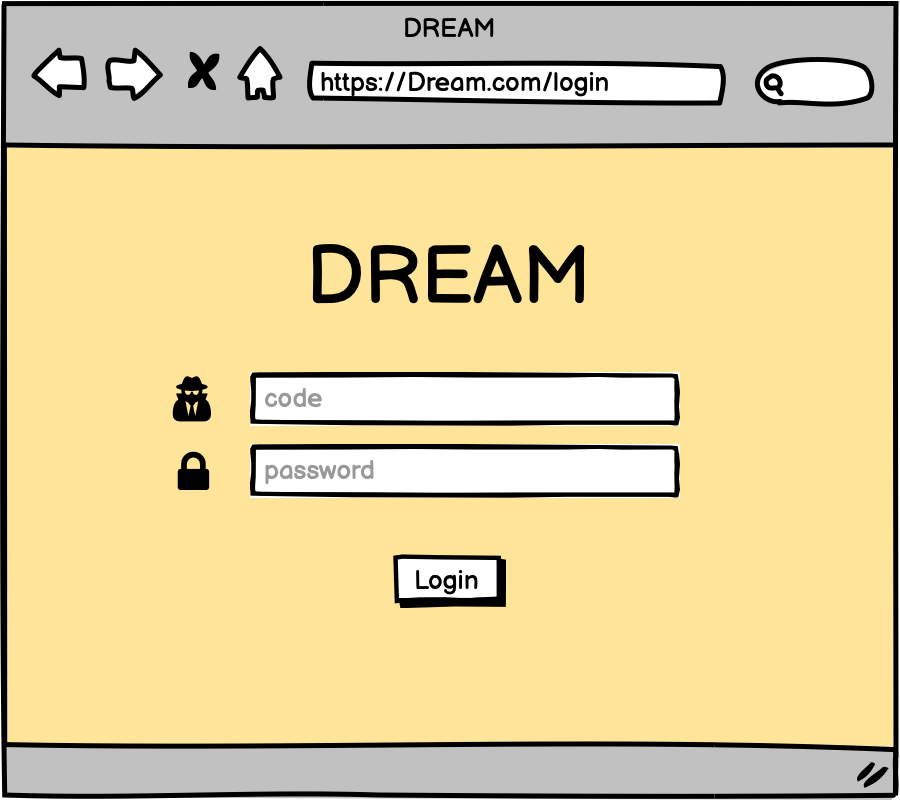
\includegraphics[width=0.7\textwidth]{mockups/PMLogIn.png}
    \caption{\emph{Policy Maker Log in} Web page}
    \label{fig:PMlogin}
    \end{center}
\end{figure}

\begin{figure}[H]
    \begin{center}
    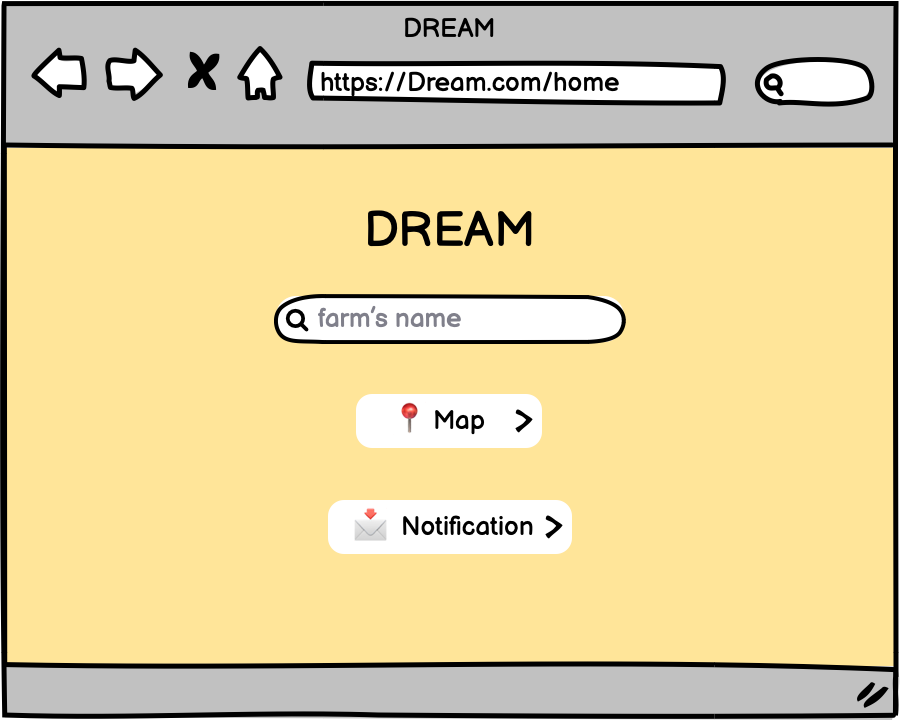
\includegraphics[width=0.7\textwidth]{mockups/PMHome.png}
    \caption{\emph{Policy Maker} Home page}
    \label{fig:PMhomepage}
    \end{center}
\end{figure}

\begin{figure}[H]
    \begin{center}
    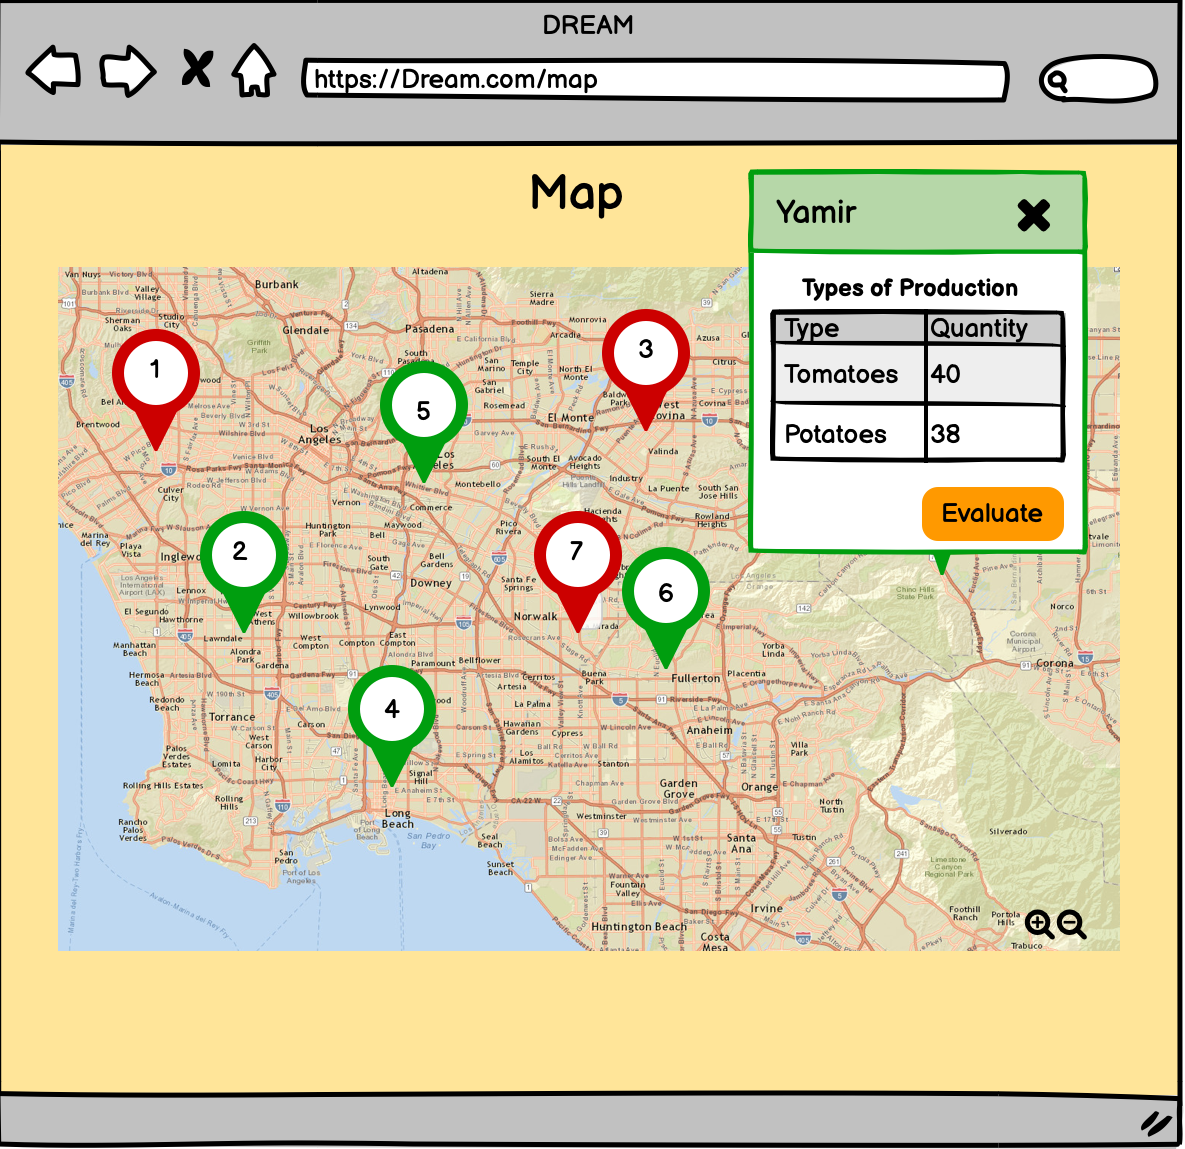
\includegraphics[width=0.7\textwidth]{mockups/PMMap.png}
    \caption{\emph{Policy Maker} Map page}
    \label{fig:PMmap}
    \end{center}
\end{figure}

\begin{figure}[H]
    \begin{center}
    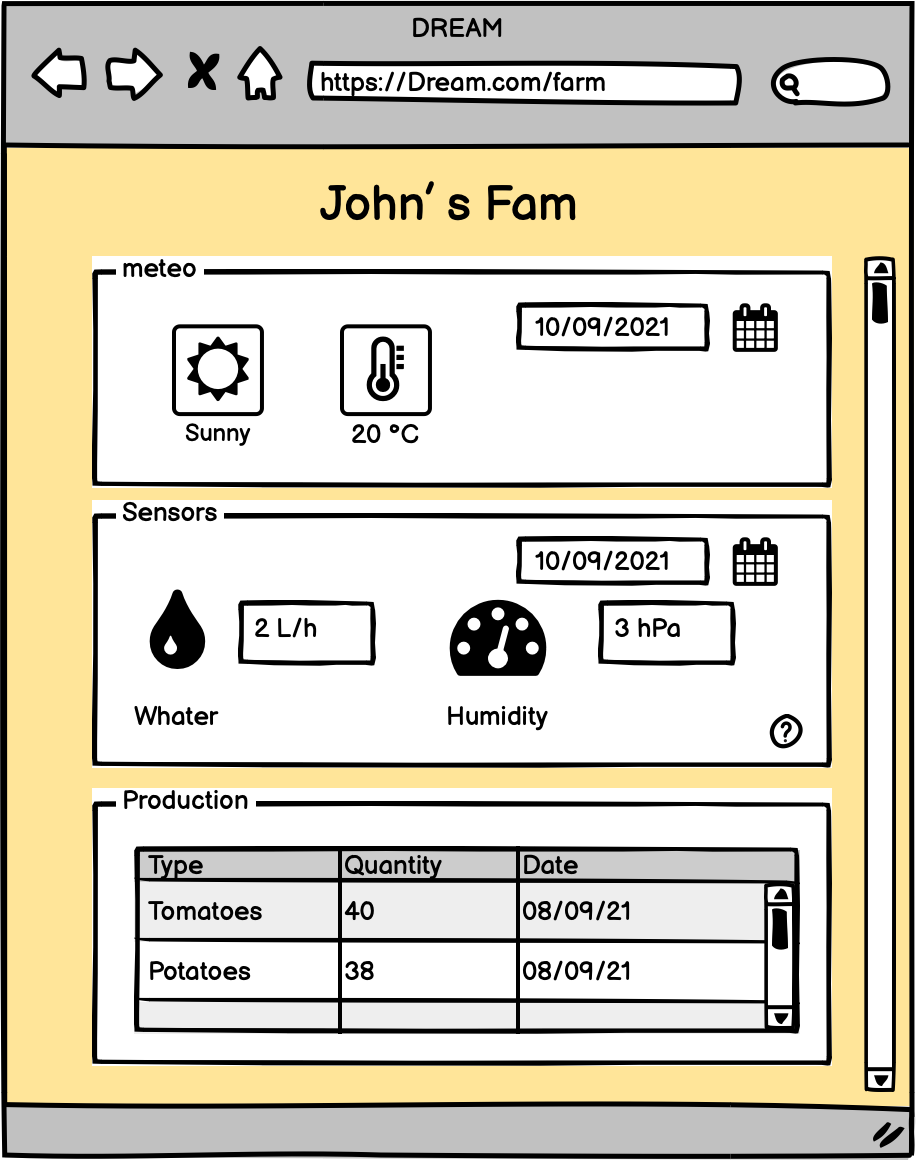
\includegraphics[width=0.7\textwidth]{mockups/PMFarm.png}
    \caption{\emph{Policy Maker} Farm's page visualization}
    \label{fig:PMFarmPage}
    \end{center}
\end{figure}

\begin{figure}[H]
    \begin{center}
    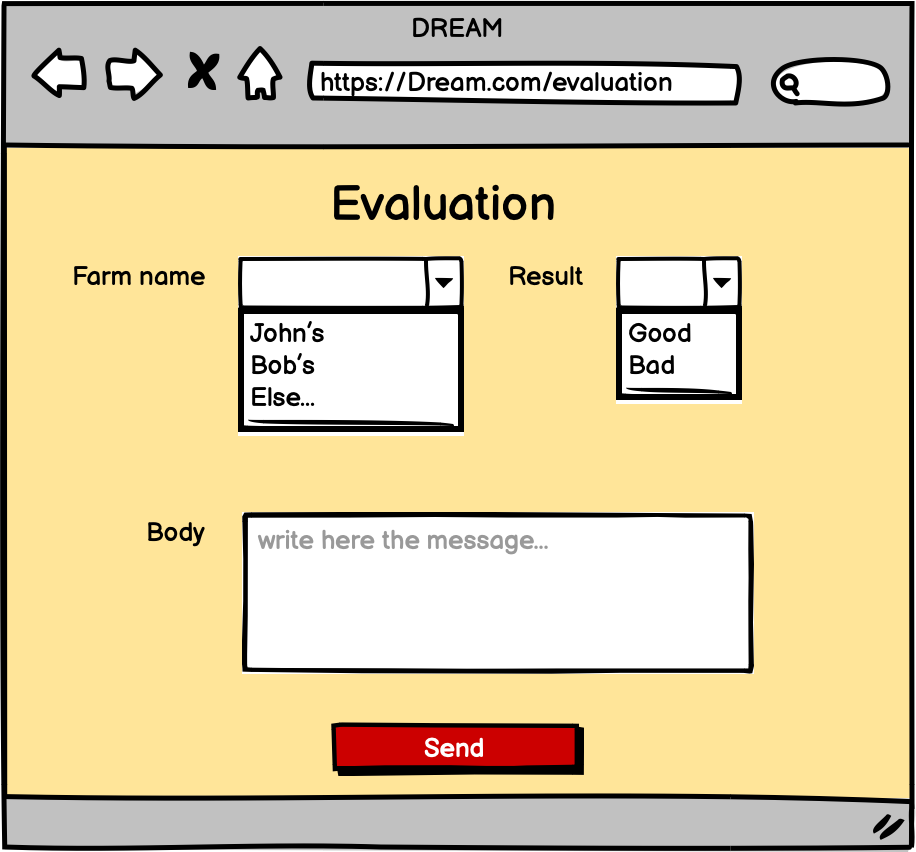
\includegraphics[width=0.7\textwidth]{mockups/Evaluation.png}
    \caption{\emph{Policy Maker} evaluation page}
    \label{fig:PMevaluation}
    \end{center}
\end{figure}

\begin{figure}[H]
    \begin{center}
    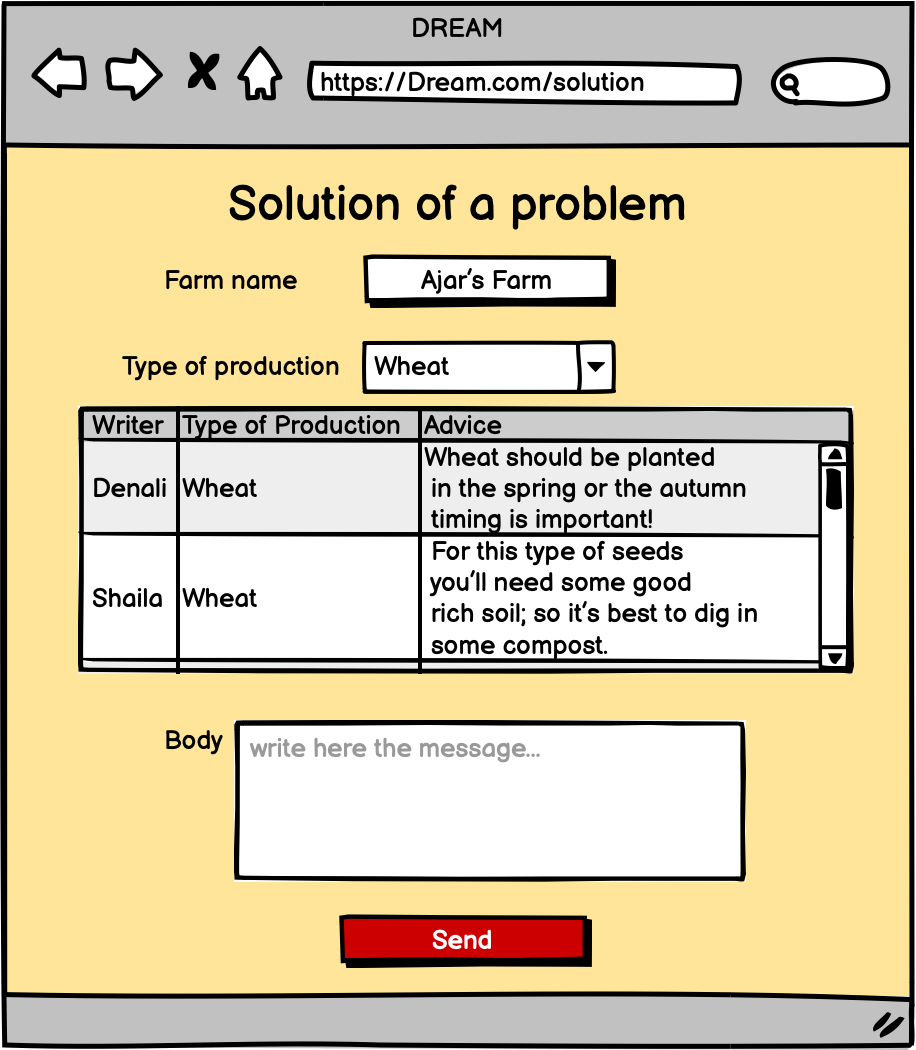
\includegraphics[width=0.7\textwidth]{mockups/Solution.png}
    \caption{\emph{Policy Maker} send solution page}
    \label{fig:PMsolution}
    \end{center}
\end{figure}

\subsubsection{Hardware Interfaces}
The application does not need any specific hardware requirements. 

\subsubsection{Software Interfaces}
The web app requires a computer with a web browser installed and connected to 
The system has to rely on a DBMS API. It allows the management of all the data the system 
needs in order to provide its functionalities, described in subsection ~\ref{subsection:2.2}.

\subsubsection{Communication Interfaces}
All the communications between users and Dream website are made via HTTPS.

\newpage

\subsection{Functional Requirements}
\subsubsection{Use Case Diagram}
\begin{figure}[H]
    \begin{center}
    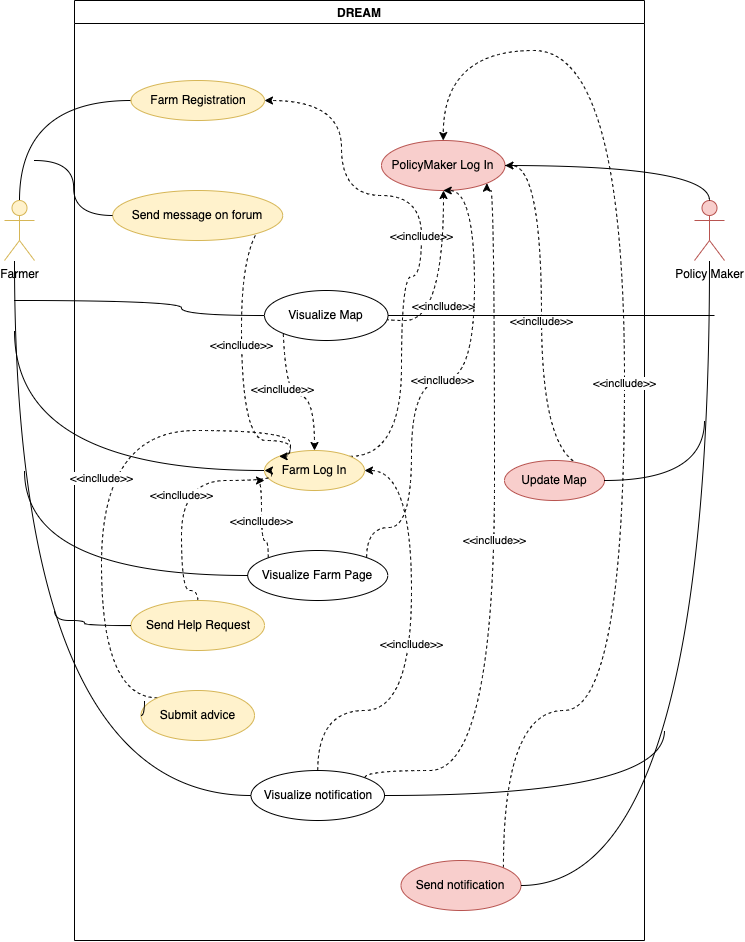
\includegraphics[width=1\textwidth]{images/useCaseDiag.drawio.png}
    \caption{Use Case diagram.}
    \label{fig:state9}
    \end{center}
\end{figure}
\subsubsection{Use Cases Description ad Sequence Diagram}
\begin{enumerate}
    \item \textbf{Farmer Registration} 
        \begin{longtable}{p{0.26\linewidth}p{0.75\linewidth}}
            \toprule
            \textbf{Name} & \textbf{Farmer Registration} \\
            \midrule
            \textbf{Actors} & Farmer \\
            \midrule
            \textbf{Entry conditions} & The web application has started\\
            \midrule
            \textbf{Flow of events} & 
            \begin{enumerate}
                \item The farmer wants to sign up
                \item The farmer inserts email, name, password, farm's name and farm's position 
                \item The farmer clicks submit
                \item The system checks if email is unique and if all the form is correctly fill up 
                \item The system inserts the information in the data base
            \end{enumerate} \\
            \midrule
            \textbf{Exit conditions} & The farmer is signed up\\
            \midrule
            \textbf{Exceptions} & 
            \begin{itemize}
                \item If the farmer did not insert data correctly the system will send an alert and let the user do that again
                \item If the email is already present in the database the system will send an alert saying that the email already exists
            \end{itemize} \\
            \bottomrule
            \caption{\emph{Farmer Registration} use case description}
        \end{longtable}
        
            \begin{figure}[H]
                \begin{center}
                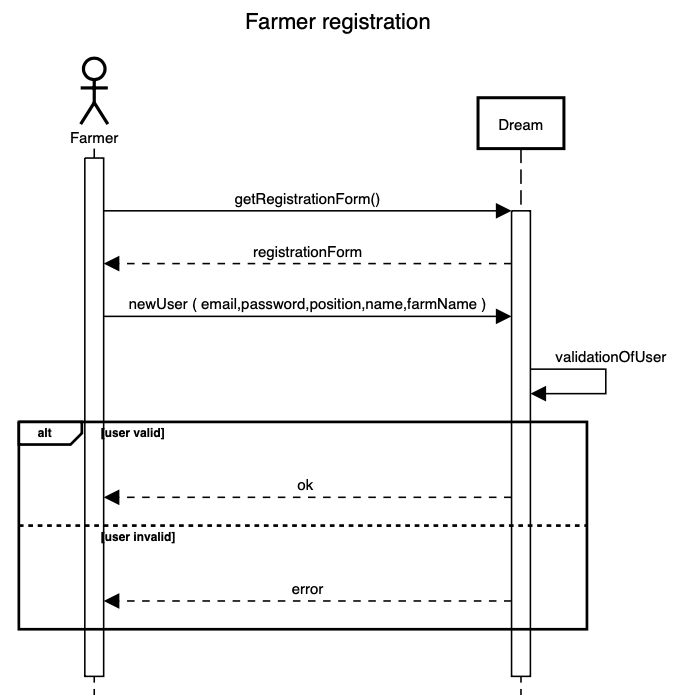
\includegraphics[width=0.7\textwidth]{sequence/FarmerRegistration.png}
                \caption{\emph{Farmer Registration} sequence diagram}
                \label{fig:sequence1}
                \end{center}
            \end{figure}

    \item \textbf{Farmer Login}
        \begin{longtable}{p{0.26\linewidth}p{0.75\linewidth}}
            \toprule
            \textbf{Name} & \textbf{Farmer Login} \\
            \midrule
            \textbf{Actors} & Farmer \\
            \midrule
            \textbf{Entry conditions} & The web application has started\\
            \midrule
            \textbf{Flow of events} & 
            \begin{enumerate}
                \item The farmer wants to log in
                \item The farmer inserts email and password
                \item The farmer clicks submit
                \item The system checks if the credentials are correct
                \item The system notifies the farmer about the correct login
            \end{enumerate} \\
            \midrule
            \textbf{Exit conditions} & The farmer has logged in\\
            \midrule
            \textbf{Exceptions} & 
            \begin{itemize}
                \item If the system does not recognize the email it will send and alert to the farmer saying that the email inserted is wrong
                \item If the password is not correct the system will notify the farmer
            \end{itemize} \\
            \bottomrule
            \caption{\emph{Farmer Login} use case description}
        \end{longtable}
        
        \begin{figure}[H]
        \begin{center}
        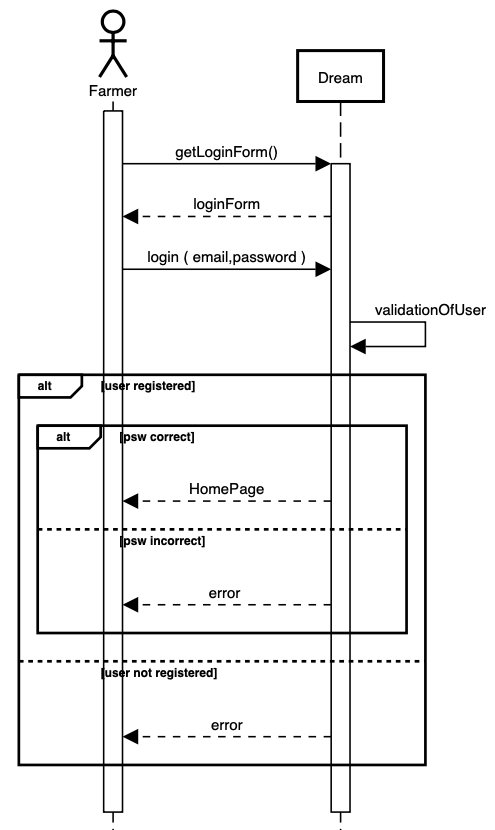
\includegraphics[width=0.5\textwidth]{sequence/FarmerLogin.png}
        \caption{\emph{Farmer Login} sequence diagram}
        \label{fig:sequence2}
        \end{center}
        \end{figure}


    \item \textbf{Farmer send a message on the Forum}
        \begin{longtable}{p{0.26\linewidth}p{0.75\linewidth}}
            \toprule
            \textbf{Name} & \textbf{Farmer sends a message on the forum} \\
            \midrule
            \textbf{Actors} & Farmer \\
            \midrule
            \textbf{Entry conditions} & The farmer has logged in\\
            \midrule
            \textbf{Flow of events} & 
            \begin{enumerate}
                \item The farmer wants to send a message
                \item The farmer clicks on forum button
                \item The system send the ser to the forum page
                \item The farmer inserts the message 
                \item The farmer clicks on send message
                \item The system inserts the message into the database 
            \end{enumerate} \\
            \midrule
            \textbf{Exit conditions} & The farmer's message is published\\
            \midrule
            \textbf{Exceptions} & 
            \begin{itemize}
                \item If the message body is empty the system shows an error alert
            \end{itemize} \\
            \bottomrule
            \caption{\emph{Farmer message} use case description}
        \end{longtable}

        \begin{figure}[H]
            \begin{center}
            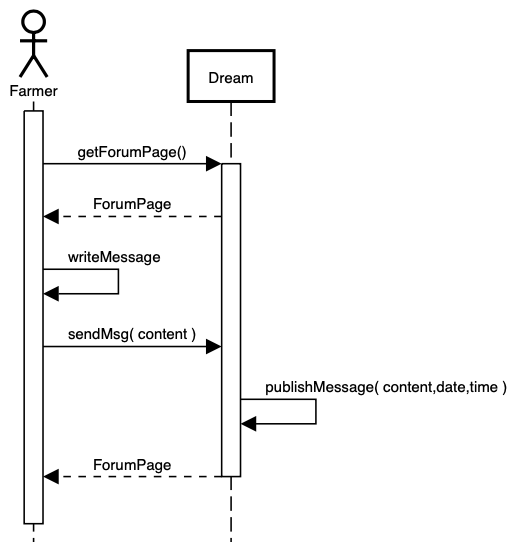
\includegraphics[width=0.6\textwidth]{sequence/messageOnForum.png}
            \caption{\emph{Farmer message} sequence diagram}
            \label{fig:sequence3}
        \end{center}
        \end{figure}

    \item \textbf{Submit production data}
        \begin{longtable}{p{0.26\linewidth}p{0.75\linewidth}}
            \toprule
            \textbf{Name} & \textbf{Farmer submit production data} \\
            \midrule
            \textbf{Actors} & Farmer \\
            \midrule
            \textbf{Entry conditions} & The farmer has logged in\\
            \midrule
            \textbf{Flow of events} & 
            \begin{enumerate}
                \item The farmer wants to add new data about his production
                \item The farmer clicks on his own farm page button
                \item The clicks on Add data button
                \item The farmer selects the type of production on which he wants to add information
                \item The farmer selects the quantity of product cultivated
                \item The farmer select the date in which he reap 
                \item The farmer clicks on submit button
                \item The system inserts the data in the database and redirect the farmer to the updated page
            \end{enumerate} \\
            \midrule
            \textbf{Exit conditions} & The farmer's data are stored\\
            \midrule
            \textbf{Exceptions} & 
            \begin{itemize}
                \item If the type of production is empty the system shows an error alert
                \item If the quantity is not specified the system shows an error alert
                \item If the date is not selected the system shows an error alert
            \end{itemize} \\
            \bottomrule
            \caption{\emph{Submit data} use case description}
        \end{longtable}

        \begin{figure}[H]
            \begin{center}
            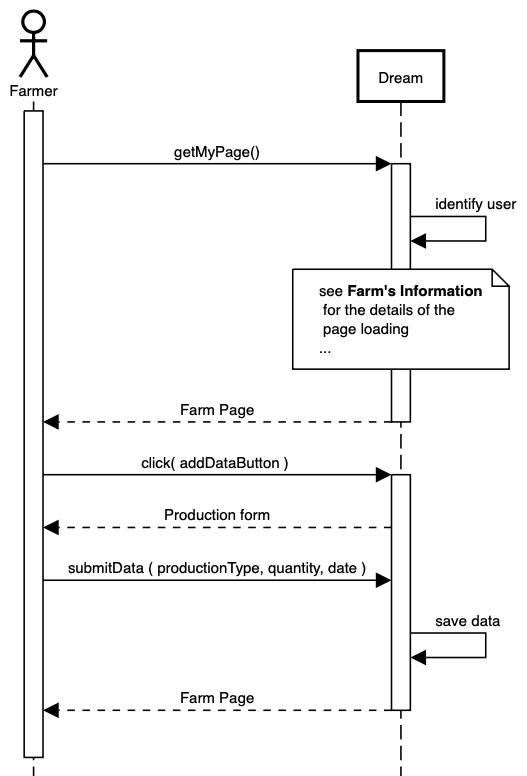
\includegraphics[width=0.6\textwidth]{sequence/AddData.png}
            \caption{\emph{Submit data} sequence diagram}
            \label{fig:sequence4}
        \end{center}
        \end{figure}
    

    \item \textbf{Find a farmer on the Map}
    \begin{longtable}{p{0.26\linewidth}p{0.75\linewidth}}
        \toprule
        \textbf{Name} & \textbf{Farmer visualizes the map} \\
        \midrule
        \textbf{Actors} & Farmer \\
        \midrule
        \textbf{Entry conditions} & The farmer has logged in\\
        \midrule
        \textbf{Flow of events} & 
        \begin{enumerate}
            \item The farmer wants to visualize the map
            \item The farmer clicks on map button
            \item The system send the farmer to the map page
            \item The farmer visualizes the map and selects a farm
            \item The system retrieves the information about the farm and shows them to the farmer
            \item The farmer visualizes the data about the selected farm
        \end{enumerate} \\
        \midrule
        \textbf{Exit conditions} & The farmer visualized the map\\
        \midrule
        \textbf{Exceptions} & \\
        \bottomrule
        \caption{\emph{Farms' map visualization} use case description}
    \end{longtable}
    \begin{figure}[H]
        \begin{center}
        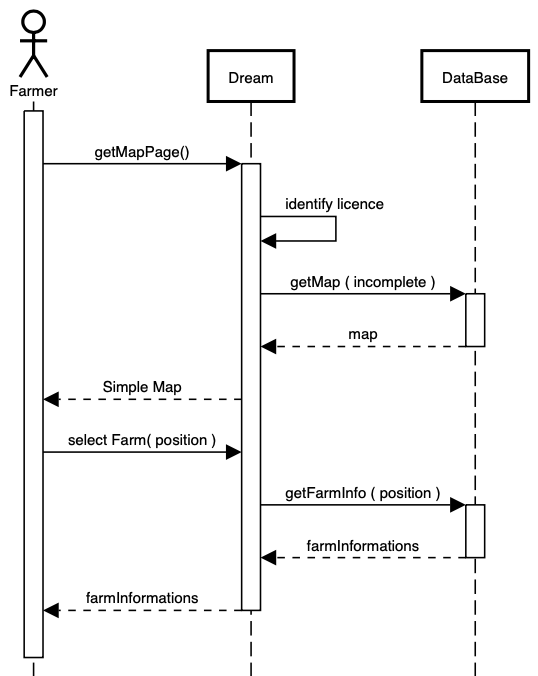
\includegraphics[width=0.45\textwidth]{sequence/VisializeMap.png}
        \caption{\emph{Farms' map visualization} sequence diagram}
        \label{fig:sequence5}
        \end{center}
    \end{figure}
    
    \item \textbf{Find farm’s information}
    \begin{longtable}{p{0.26\linewidth}p{0.75\linewidth}}
        \toprule
        \textbf{Name} & \textbf{Farmer visualizes their own data} \\
        \midrule
        \textbf{Actors} & Farmer \\
        \midrule
        \textbf{Entry conditions} & The farmer has logged in\\
        \midrule
        \textbf{Flow of events} & 
        \begin{enumerate}
            \item The farmer wants to visualize his own page
            \item The farmer clicks on the profile page button
            \item The system retrives the information about the farmer and redirect him to the farmer's farm page
            \item The farmer visualizes his own page
        \end{enumerate} \\
        \midrule
        \textbf{Exit conditions} & The farmer visualizes his own data\\
        \midrule
        \textbf{Exceptions} & 
        \begin{enumerate}
            \item
        \end{enumerate}\\
        \bottomrule
        \caption{\emph{Farm information visualization} use case description}
    \end{longtable}

    \begin{figure}[H]
        \begin{center}
        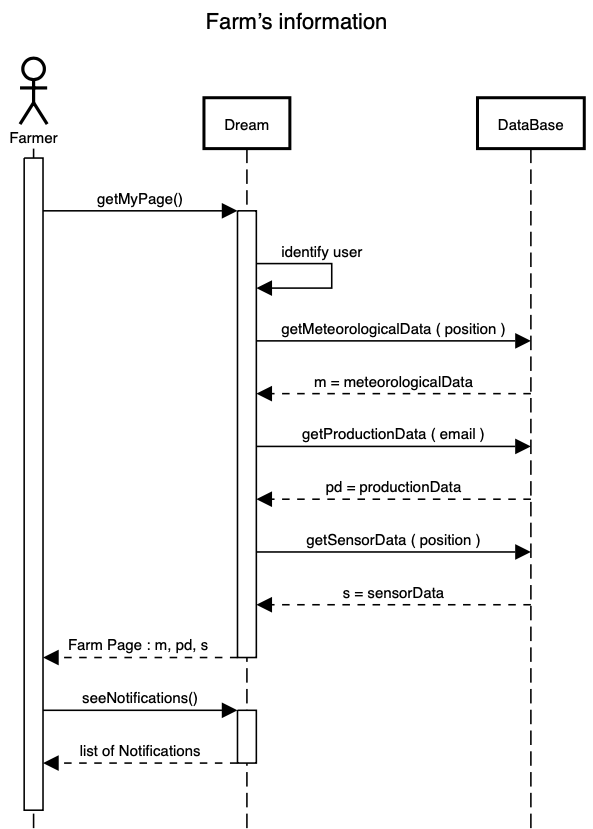
\includegraphics[width=0.7\textwidth]{sequence/FarmInformation.png}
        \caption{\emph{Farm information visualization} sequence diagram}
        \label{fig:sequence6}
        \end{center}
    \end{figure}

    \item \textbf{Submit a request of help}
    \textbf{I put only the case of a forml request to the Policy Maker (button on Farm Page) if you want we can create 2 "secion" (alt) one with this formal request and one sending a message on Forum (but is yet specified in 3)}
    \begin{longtable}{p{0.26\linewidth}p{0.75\linewidth}}
        \toprule
        \textbf{Name} & \textbf{Farmer submit a request of help} \\
        \midrule
        \textbf{Actors} & Farmer \\
        \midrule
        \textbf{Entry conditions} & The farmer has logged in\\
        \midrule
        \textbf{Flow of events} & 
        \begin{enumerate}
            \item The farmer wants to ask for help
            \item The farmer clicks on his own page button
            \item The farmer clicks on Help button
            \item The farmer chooses the type of production on which he had problems
            \item The farmer fills the form specifying the problem
            \item The farmer clicks on the submit button and sends the message
            \item The system sends the notification to the Policy Makers
            \item The system notifies the farmer that the operation went succesfully
            \item The system returns a list of advices retrieved from the database about the type of production selected
        \end{enumerate} \\
        \midrule
        \textbf{Exit conditions} & The help request is sent to the Policy Makers\\
        \midrule
        \textbf{Exceptions} & 
        \begin{itemize}
            \item If no type of production is selected the system notifies the farmer and waits for him to insert it
            \item If the request body is empty the system notifies the farmer and waits for him to fill it in
        \end{itemize}\\
        \bottomrule
        \caption{\emph{Farmer ask for help} use case description}
    \end{longtable}

    \begin{figure}[H]
        \begin{center}
        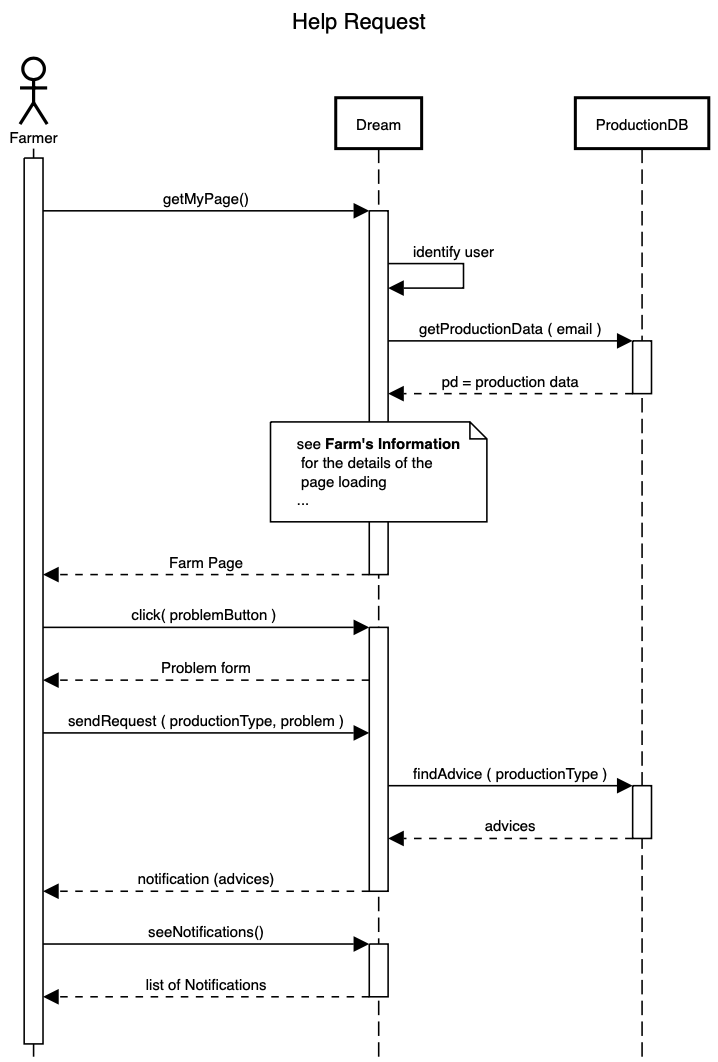
\includegraphics[width=0.7\textwidth]{sequence/HelpRequest.png}
        \caption{\emph{Farmer ask for help} sequence diagram}
        \label{fig:sequence7}
        \end{center}
    \end{figure}

    \item \textbf{Submit an advice}
    \begin{longtable}{p{0.26\linewidth}p{0.75\linewidth}}
        \toprule
        \textbf{Name} & \textbf{Farmer submits an advice} \\
        \midrule
        \textbf{Actors} & Farmer \\
        \midrule
        \textbf{Entry conditions} & The farmer has logged in\\
        \midrule
        \textbf{Flow of events} & 
        \begin{enumerate}
            \item The farmer has to submit an advice 
            \item The farmer clicks on his own page button
            \item The farmer clicks on Advice button
            \item The farmer chooses the type of production on which he wants to give advices
            \item The farmer fills the form writing his advice
            \item The farmer clicks submit button and sends the message
            \item The system saves the advice in the database
            \item The system notifies the farmer that the operation went succesfully 
        \end{enumerate} \\
        \midrule
        \textbf{Exit conditions} & The farmer submit an advice\\
        \midrule
        \textbf{Exceptions} & 
        \begin{itemize}
            \item If the farmer is not a "good" one the system doesn't save the advice and nottifies the farmer with an error message
        \end{itemize}\\
        \bottomrule
        \caption{\emph{Farmer send advice} use case description}
    \end{longtable}

    \begin{figure}[H]
        \begin{center}
        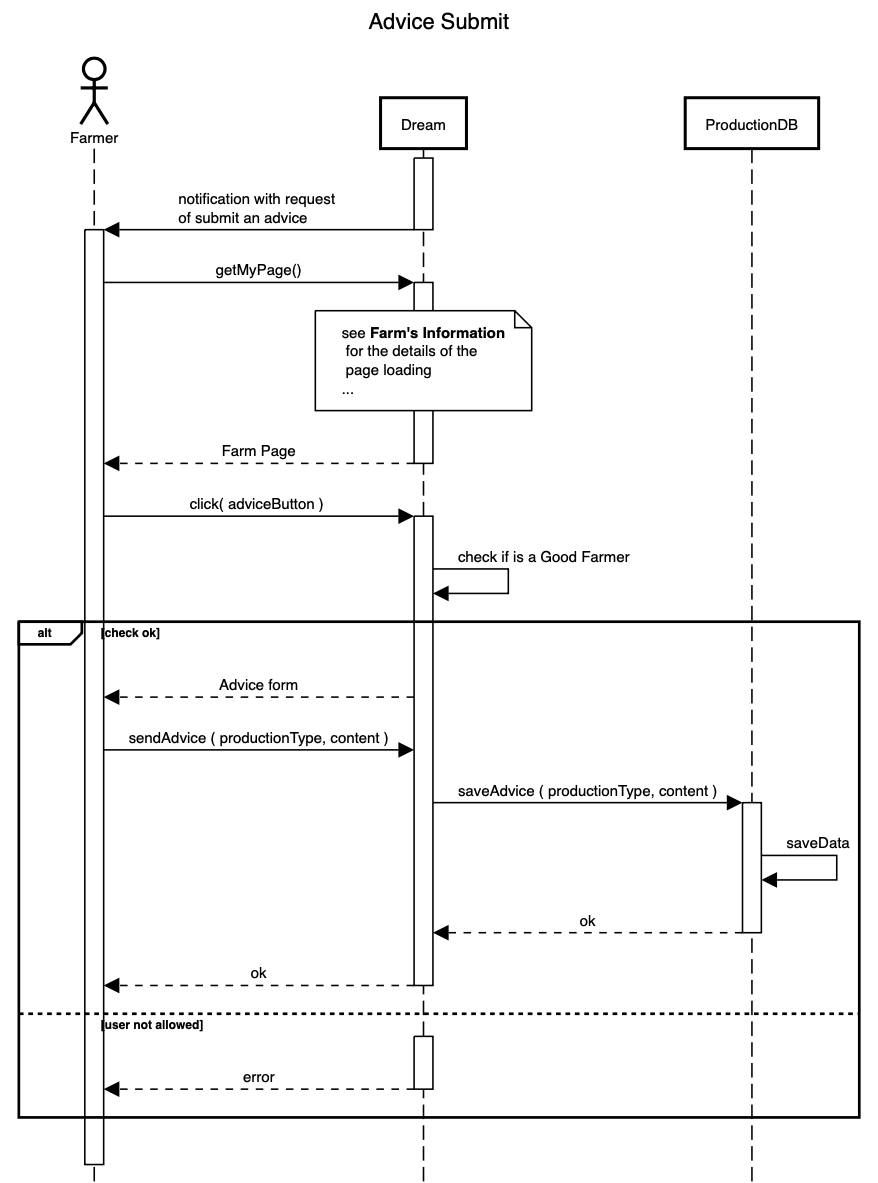
\includegraphics[width=0.7\textwidth]{sequence/AdviceSubmit.png}
        \caption{\emph{Farmer send advice} sequence diagram}
        \label{fig:sequence8}
        \end{center}
    \end{figure}

    \item \textbf{Visualize notifications}
    \begin{longtable}{p{0.26\linewidth}p{0.75\linewidth}}
        \toprule
        \textbf{Name} & \textbf{Farmer visualizes his notifications} \\
        \midrule
        \textbf{Actors} & Farmer \\
        \midrule
        \textbf{Entry conditions} & The farmer has logged in\\
        \midrule
        \textbf{Flow of events} & 
        \begin{enumerate}
            \item The farmer wants to read his notifications
            \item The farmer clicks on his own page button
            \item The farmer clicks on Notification button
            \item The system returns a list of messages
            \item The farmer selects one message between the ones in the list
            \item The system returns the body of the message
        \end{enumerate} \\
        \midrule
        \textbf{Exit conditions} & The farmer visualizes his notifications\\
        \midrule
        \textbf{Exceptions} & 
        \begin{itemize}
            \item 
        \end{itemize}\\
        \bottomrule
        \caption{\emph{Farmer visualize notifications} use case description}
    \end{longtable}

    \begin{figure}[H]
        \begin{center}
        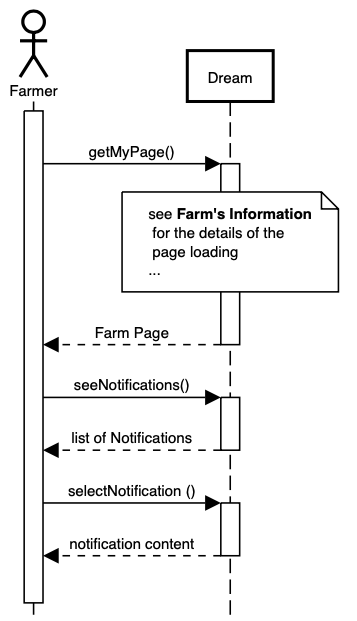
\includegraphics[width=0.7\textwidth]{sequence/SeeNotifications.png}
        \caption{\emph{Farmer visualize notifications} sequence diagram}
        \label{fig:sequence9}
        \end{center}
    \end{figure}

    \item \textbf{Policy Maker login}
    \begin{longtable}{p{0.26\linewidth}p{0.75\linewidth}}
        \toprule
        \textbf{Name} & \textbf{Farmer visualizes their own data} \\
        \midrule
        \textbf{Actors} & Policy Maker \\
        \midrule
        \textbf{Entry conditions} & The web application has started\\
        \midrule
        \textbf{Flow of events} & 
        \begin{enumerate}
            \item The Policy Maker wants to log in 
            \item The Policy Maker inserts code and password
            \item The Policy Maker clicks the submit button
            \item The system checks if the credentials are correct
            \item The system notifies the Policy Maker about the correct login
        \end{enumerate} \\
        \midrule
        \textbf{Exit conditions} & The Policy Maker has logged in\\
        \midrule
        \textbf{Exceptions} & 
        \begin{itemize}
            \item If the system does not recognize the code it will send an alert  to the Policy Maker saying that the code inserted is wrong
            \item If the password is not correct the system will notify the Policy Maker 
        \end{itemize}\\
        \bottomrule
        \caption{\emph{Policy Maker login} use case description}
    \end{longtable}

    \begin{figure}[H]
        \begin{center}
        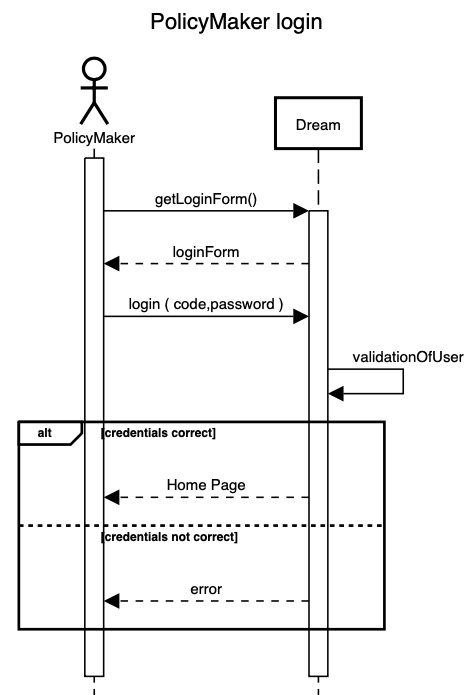
\includegraphics[width=0.7\textwidth]{sequence/PolicyMakerLogin.png}
        \caption{\emph{Policy Maker login} sequence diagram}
        \label{fig:sequence10}
        \end{center}
    \end{figure}

    \item \textbf{Find a farm's page}
    \begin{longtable}{p{0.26\linewidth}p{0.75\linewidth}}
        \toprule
        \textbf{Name} & \textbf{Policy Maker visualizes a farm’s page} \\
        \midrule
        \textbf{Actors} & Policy Maker \\
        \midrule
        \textbf{Entry conditions} & The Policy Maker has logged in\\
        \midrule
        \textbf{Flow of events} & 
        \begin{enumerate}
            \item The Policy Maker wants to visualize a farm's page
            \item The Policy Maker types the name of the farm on the search form
            \item The Policy Maker clicks search button
            \item The system redirects the Policy Maker to the farm's page
        \end{enumerate} \\
        \midrule
        \textbf{Exit conditions} & The Policy Maker visualizes the farm's page\\
        \midrule
        \textbf{Exceptions} & 
        \begin{itemize}
            \item If no name is inserted in the search form the system notifies the Policy Maker about the missing data
            \item If the name inserted is not present in the system's database, the system sends an error message
        \end{itemize}\\
        \bottomrule
        \caption{\emph{Farm’s page visualization} use case description}
    \end{longtable}

    \begin{figure}[H]
        \begin{center}
        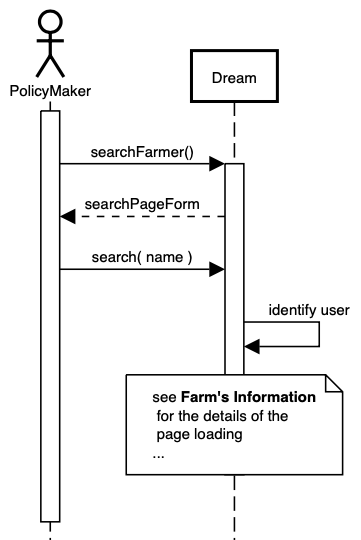
\includegraphics[width=0.7\textwidth]{sequence/PolicyMakerseachFarm.png}
        \caption{\emph{Farm’s page visualization} sequence diagram}
        \label{fig:sequence11}
        \end{center}
    \end{figure}

    \item \textbf{Find a farmer on the Map}
    \begin{longtable}{p{0.26\linewidth}p{0.75\linewidth}}
        \toprule
        \textbf{Name} & \textbf{Policy Maker visualizes a farm’s page} \\
        \midrule
        \textbf{Actors} & Policy Maker \\
        \midrule
        \textbf{Entry conditions} & The Policy Maker has logged in\\
        \midrule
        \textbf{Flow of events} & 
        \begin{enumerate}
            \item The Policy Maker wants to visualize the map
            \item The Policy Maker clicks on map button
            \item The system redirects the Policy Maker to the map page
            \item The Policy Maker visualizes the map and selects a farm
            \item The system retrieves the information about the farm (also the last evaluation) and shows them to the Policy Maker
            \item The Policy Maker visualizes the data about the selected farm
        \end{enumerate} \\
        \midrule
        \textbf{Exit conditions} & The Policy Maker visualizes his own data\\
        \midrule
        \textbf{Exceptions} & 
        \begin{itemize}
            \item 
        \end{itemize}\\
        \bottomrule
        \caption{\emph{Farm visualization on map} use case description}
    \end{longtable}

    \begin{figure}[H]
        \begin{center}
        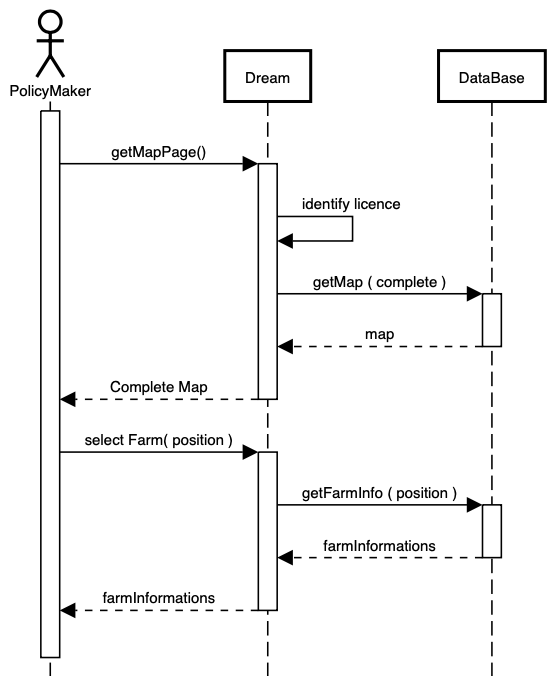
\includegraphics[width=0.7\textwidth]{sequence/searchOnMap.png}
        \caption{\emph{Farm visualization on map} sequence diagram}
        \label{fig:sequence12}
        \end{center}
    \end{figure}

    \item \textbf{Update the Map}
    \begin{longtable}{p{0.26\linewidth}p{0.75\linewidth}}
        \toprule
        \textbf{Name} & \textbf{Policy Maker update the map} \\
        \midrule
        \textbf{Actors} & Policy Maker \\
        \midrule
        \textbf{Entry conditions} & The Policy Maker has logged in\\
        \midrule
        \textbf{Flow of events} & 
        \begin{enumerate}
            \item The Policy Maker wants to report an evaluation
            \item The Policy Maker clicks on the map button
            \item The system redirects the Policy Maker to the map page
            \item The Policy Maker visualizes the map and selects a farm
            \item The system retrieves the information about the farm (also the last evaluation) and shows them to the Policy Maker
            \item The Policy Maker clicks update button
            \item The Policy Maker select the evaluation
                \begin{itemize}
                    \item The Policy Maker selects "good", decides an amount of money for the award and writes the body of the message
                    \item The Policy Maker selects "bad" and writes the body of the message
                \end{itemize}
            \item The Policy Maker clicks submit button and sends the message
            \item The system saves the evaluation on the map
            \item The system sends the message to the Farm's owner
            \item The system notifies the Policy Maker that the operation went succesfully 
        \end{enumerate} \\
        \midrule
        \textbf{Exit conditions} & The Policy Maker visualizes the map updated\\
        \midrule
        \textbf{Exceptions} & 
        \begin{itemize}
            \item 
        \end{itemize}\\
        \bottomrule
        \caption{\emph{Map updating} use case description}
    \end{longtable}

    \begin{figure}[H]
        \begin{center}
        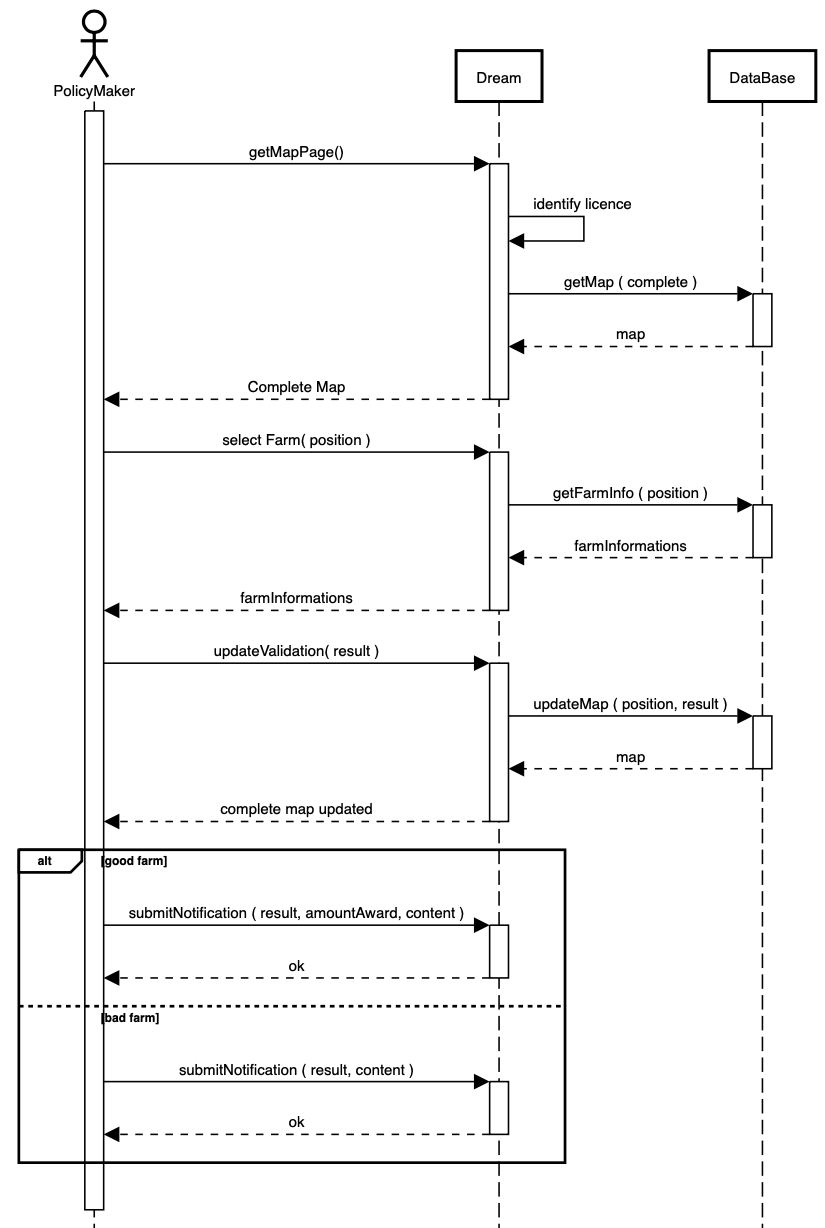
\includegraphics[width=0.7\textwidth]{sequence/updateMap.png}
        \caption{\emph{Map updating} sequence diagram}
        \label{fig:sequence13}
        \end{center}
    \end{figure}

    \item \textbf{Reply to a request of help}
    \begin{longtable}{p{0.26\linewidth}p{0.75\linewidth}}
        \toprule
        \textbf{Name} & \textbf{Policy Maker send anvice} \\
        \midrule
        \textbf{Actors} & Policy Maker \\
        \midrule
        \textbf{Entry conditions} & The Policy Maker has logged in\\
        \midrule
        \textbf{Flow of events} & 
        \begin{enumerate}
            \item The Policy Maker wants to send specific advices to a farmer
            \item The Policy Maker wants to see the informationabout a farm
            \item The Policy Maker types the name of the farm on search form
            \item The Policy Maker clicks search button 
            \item The Policy Maker wants to see the advices stored in the database on the type of production the farmers asked for help on
            \item The Policy Maker analyzes the data 
            \item The Policy Maker selects the farmer (name) and the type of production and writes the solution he found
            \item The Policy Maker clicks send button
            \item The system sends the message to the farmer
            \item The system notifies the Policy Maker that the operation was succesful
        \end{enumerate} \\
        \midrule
        \textbf{Exit conditions} & The Policy Maker send solutions\\
        \midrule
        \textbf{Exceptions} & 
        \begin{itemize}
            \item 
        \end{itemize}\\
        \bottomrule
        \caption{\emph{Problem resolution} use case description}
    \end{longtable}

    \begin{figure}[H]
        \begin{center}
        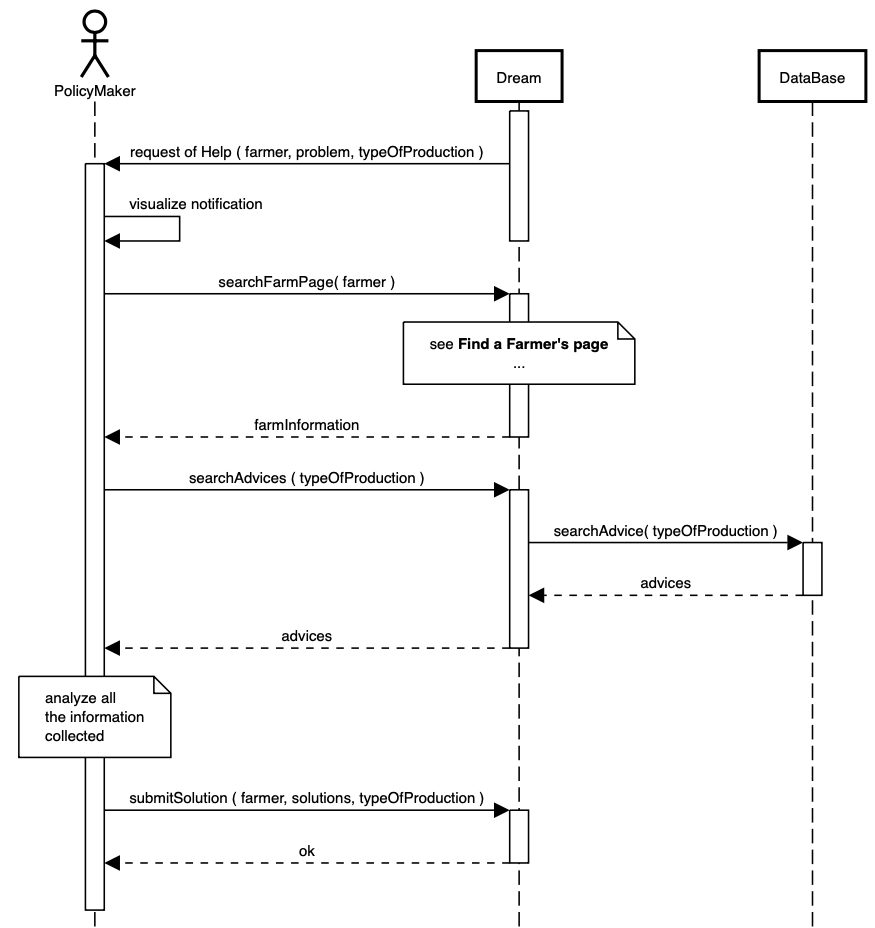
\includegraphics[width=0.7\textwidth]{sequence/replyHelp.png}
        \caption{\emph{Problem resolution} sequence diagram}
        \label{fig:sequence14}
        \end{center}
    \end{figure}
\end{enumerate}

%-----------------------------------------------------------------------------------%
\subsubsection{Scenarios}
\begin{enumerate}
    \item \textbf{Scenario 1}\\
    Dayanita is a young woman that lives in Singaram, a small town in the state of Telengana in India. 
    She lives with her parents in their family's farm. \\
    Their farm was mostly used to cultivate rice, so they are not really expert in other types of crop. She decides to try to expand their business, starting to grow 
    soyabean but her parents do not really know how to help her with it. \\
    Dayanita discovers, thanks to an ad she found online, a new web application that has been recently released. \\
    Therefore she decides to sign up and write a message on the forum hoping that some other farmer can share with her some advices.\\
    Ajar, the owner of Ajar's farm, answered her message saying to be careful and check the weather condition before planting the seeds and some suggestions 
    about the appropriate depth for planting them. 
    Dayainita some days later checks the forum again and reads Ajar's message. 
    The following days she checks the weather forecast that is present on her personalized farm page and actually 
    finds the right period to start planting soyabean.



    \item \textbf{Scenario 2}\\
    Nanuk is a Telengana’s policy maker. Dream IT providers distributed to each policy maker 
    reported by Telengana's government a secret code. Through this code 
    and password Nanuk is able to log in to Dream web application. 
    Before the 10th of the month all the policy makers are suppose to update the past evaluation 
    of the farms already present in 
    the system and add the farms that are added in the system in the past month.
    Using Dream the Nanuk searches on the map the farms that already been evaluated last month. 
    He finds out that Shaila's Farm did 
    not perform that well last time it was evaluated.
    Thus he decides to see if her performance is improved in the last month, he check the quantity 
    of wheat producted and 
    saw it increased dramatically from the month before.
    Therefore he decides to classify the farm as GOOD with a small incentive so that the owner 
    of the farm is stimulated to keep on doing good.
    
    
    \item \textbf{Scenario 3}\\
    Yamir is struggling with his Sesame crop. He tried everything, but still can not grow a quantity 
    that could increase his profit. \\
    His friend Ishaan only grows corn so he said he could not help him with it. However he suggested him to try to sign up to Dream 
    saying that there are a lot of ways he could get support from there. \\
    After he signed up he tried to write a message on the forum but nobody answered his text. 
    So he sent a request of help to the policy makers and finally discovered that he need to give more water to his plants.

    \item \textbf{Scenario 4}\\
    A policy maker working for Telengana's government is working with Dream application. The policy maker logs in with his code and password 
    to check his notification. \\
    The first notification he notices is a new request of help from Ajar's farm. He then looks at Ajar's farm page to look up all the information.\\
    Ajar is looking for suggestions on his wheat crop. The policy maker at this point send the solution of Ajar's problem, 
    filtering for type of production: wheat. 
    He reads all the advices written by other farmers and chooses the one written by Denali: wheat should be 
    planted in autumn or spring not in the other seasons. The policy maker writes then the solution and sends it to the farmer Ajar.

    
    
\end{enumerate}


%-----------------------------------------------------------------------------------%
\subsubsection{Requirements}
\textbf{R1} The system must allow farmers to register\\
\textbf{R2} The system must allow farmers to log in\\
\textbf{R3} The system must save the farmers registration data\\
\textbf{R4} The system must guarantee that each email address is unique\\
\textbf{R5} The system must verify that the email address is valid (the type!)\\
\textbf{R6} The system must save the farmers information about their production submitted\\
\textbf{R7} The system must allow farmers to insert the type of production \\
\textbf{R8} The system must allow farmers to insert the amount of production type\\
\textbf{R9} The system must allow farmers to specify a problem they faced to the Policy Makers\\
\textbf{R10} The system must allow farmers to select the type of production on which they had troubles\\
\textbf{R11} The system must save the advice submitted by the farmers\\
\textbf{R12} The system must allow farmers to select the type of product in their suggestion\\
\textbf{R13} The system must be able to show to the farmers advices send by the Policy Makers (as a notification)\\
\textbf{R14} The system must be able to show the meteorological data of the Farm’s position\\
\textbf{R15} The system must be able to show the farm’s sensor data \\
\textbf{R16} The system must allow farmers to send messages on the forum\\
\textbf{R17} The system must register date and time of a message in the forum\\
\textbf{R18} The system must be able to show all the messages on the forum\\
\textbf{R19} The system must be able to show the map of the zone\\
\textbf{R20} The system must be able to show the farms position on the map\\
\textbf{R21} the system must be able to show on the map if a farm is performing well or not \\
\textbf{R22} The system must allow farmers to visualise notification send by Policy Makers\\
\textbf{R23} The system must allow farmers to see all information about his own farm\\
\textbf{R24} The system must be able to show the types of production cultivated in a farm\\
\textbf{R25} The system must be able to show the quantity of product has been cultivated for each type in a farm\\
\textbf{R26} The system does not allow Policy Makers to register\\
\textbf{R27} The system must allow Policy Makers to log in\\
\textbf{R28} The system must verify that the code is valid\\
\textbf{R29} The system must allow Policy Makers to search a farm by name\\
\textbf{R30} The system must allow Policy Makers to see all farms’ pages\\
\textbf{R31} The system must not allow Policy Makers to modify any farm page\\
\textbf{R32} The system must allow Policy Makers to update the performance of a farmer\\
\textbf{R33} The system must allow Policy Makers to send notifications to the farmers\\
\textbf{R34} The system must allow Policy Makers to receive requests of help by the farmers\\
%-----------------------------------------------------------------------------------%
\newpage

\subsubsection{Goals}

\begin{table}[ht]

\begin{center}

\begin{tabular}{|p{2cm}|p{4cm}|p{4cm}|}
    
    \toprule
   Goals & Domain Assumpitons & Requirements \\
   \midrule
    G1 & DA1, DA2, DA3, DA4, DA5, DA6, DA7, DA8, DA9, DA13, DA16, DA18 & R14, R15, R26, R27, R28, R29, R30, R31, R32 \\ 
    \midrule
    G2 & DA1, DA4, DA6, DA10, DA15, DA17 & R1, R2, R3, R4, R5, R16, R17, R18 \\
    \midrule
    G3 & DA1, DA2, DA6, DA9, DA12, DA14, DA15, DA17 & R1, R2, R3, R4, R5, R6, R7, R8, R11, R12 \\
    \midrule
    G4 & DA1, DA6, DA9, DA11, DA15, DA17 & R1, R2, R3, R4, R5, R9, R10, R13, R22, R33, R34 \\
    \midrule
    G5 & DA1, DA3, DA4, DA5, DA6, DA7, DA8, DA9, DA10, DA13, DA15, DA17 & R1, R2, R3, R4, R5, R14, R15, R22, R23, R24, R25 \\
    \midrule
    G6A & DA1, DA5, DA6, DA8, DA9, DA15, DA16, DA17 & R1, R2, R3, R4, R5, R19, R20, R26, R27, R28 \\
    \midrule
    G6B & DA1, DA2, DA5, DA6, DA8, DA9, DA13, DA15, DA16, DA17 & R19, R20, R21, R24, R25, R26, R27, R28, R32, R33 \\
    \midrule
    G6C & DA1, DA2, DA5, DA6, DA8, DA9, DA15, DA16, DA17 & R1, R2, R3, R4, R5, R19, R20, R24 \\
    \bottomrule
\end{tabular}
\end{center}
\caption{Mapping of goals, domain assumptions and requirements}
\end{table}



\begin{itemize}   
    \item \textbf{G1} Allow Policy Makers to retrieve information about a farm and to evaluate their performance
        \begin{itemize}
            \renewcommand\labelitemi{--}
            \item \textbf{R14} The system must be able to show the meteorological data of the Farm’s position
            \item \textbf{R15} The system must be able to show the farm’s sensor data
            \item \textbf{R26} The system does not allow Policy Makers to register
            \item \textbf{R27} The system must allow Policy Makers to log in
            \item \textbf{R28} The system must verify that the code is valid
            \item \textbf{R29} The system must allow Policy Makers to search a farm by name
            \item \textbf{R30} The system must allow Policy Makers to see all farms’ pages
            \item \textbf{R31} The system must not allow Policy Makers to modify any farm’s page
            \item \textbf{R32} The system must allow Policy Makers to update the performance of a farmer
            \item \textbf{DA1} In order to access the system users need to have Internet connection
            \item \textbf{DA2} Farmers always insert correct data on their production activity
            \item \textbf{DA3} Data from sensors is always correct
            \item \textbf{DA4} Date and Time on the system are always correct
            \item \textbf{DA5} The position of the Farm is always correct
            \item \textbf{DA6} Internet connection works always without errors
            \item \textbf{DA7} Meteorological data is accurate
            \item \textbf{DA8} Every farm has a different position
            \item \textbf{DA9} Each farm belongs to exacly one farmer
            \item \textbf{DA13} Performances of farmers are always identified correctly
            \item \textbf{DA16} Policy Makers have a given code and password to access the system
            \item \textbf{DA18} The special incentive that the farmers receive for their good work, is used on stuff related to their farm activity
        \end{itemize}
    
    \item \textbf{G2} Allow farmer to comunicate with each other
        \begin{itemize}
            \renewcommand\labelitemi{--}
            \item \textbf{R1} The system must allow farmers to register
            \item \textbf{R2} The system must allow farmers to log in
            \item \textbf{R3} The system must save the farmers registration data
            \item \textbf{R4} The system must guarantee that each email address is unique
            \item \textbf{R5} The system must verify that the email address is valid
            \item \textbf{R16} The system must allow farmers to send messages on the forum
            \item \textbf{R17} The system must register date and time of a message in the forum
            \item \textbf{R18} The system must be able to show all messages on the forum
            \item \textbf{DA1} In order to access the system users need to have Internet connection
            \item \textbf{DA4} Date and Time on the system are always correct
            \item \textbf{DA6} Internet connection works always without errors
            \item \textbf{DA10} Discussion on the forum are related only to the farm activity
            \item \textbf{DA15} The email and farm's name must be unique
            \item \textbf{DA17} All farmers that sign up own a real farm in Telengana
        \end{itemize}    
    
    \item \textbf{G3} Allow farmer to insert data and advices on his production
        \begin{itemize}
        \renewcommand\labelitemi{--}
        \item \textbf{R1} The system must allow farmers to register
        \item \textbf{R2} The system must allow farmers to log in
        \item \textbf{R3} The system must save the farmers registration data
        \item \textbf{R4} The system must guarantee that each email address is unique
        \item \textbf{R5} The system must verify that the email address is valid
        \item \textbf{R6} The system must save the farmers information about their production submitted
        \item \textbf{R7} The system must allow farmers to insert the type of production
        \item \textbf{R8} The system must allow farmers to insert the amount of production type
        \item \textbf{R11} The system must save the advice submitted by the farmers
        \item \textbf{R12} The system must allow farmers to select the type of product in their suggestion
        \item \textbf{DA1} In order to access the system users need to have Internet connection
        \item \textbf{DA2} Farmers always insert correct data on their production activity
        \item \textbf{DA6} Internet connection works always without errors
        \item \textbf{DA9} Each farm belongs to exacly one farmer
        \item \textbf{DA12} Advice on a product must be given by a farmer that produces the same type
        \item \textbf{DA14} Farmers can insert data more than once a day
        \item \textbf{DA15} The email and farm's name must be unique
        \item \textbf{DA17} All farmers that sign up own a real farm in Telengana
        \end{itemize} 
    
    \item \textbf{G4} Allow farmer to send request of help to Policy Makers
        \begin{itemize}
        \renewcommand\labelitemi{--}
        \item \textbf{R1} The system must allow farmers to register
        \item \textbf{R2} The system must allow farmers to log in
        \item \textbf{R3} The system must save the farmers registration data
        \item \textbf{R4} The system must guarantee that each email address is unique
        \item \textbf{R5} The system must verify that the email address is valid
        \item \textbf{R9} The system must allow farmers to specify a problem they faced to the Policy Makers
        \item \textbf{R10} The system must allow farmers to select the type of production on which they had troubles
        \item \textbf{R13} The system must be able to show to the farmers advices send by the Policy Makers
        \item \textbf{R22} The system must allow farmers to visualise notification send by Policy Makers
        \item \textbf{R33} The system must allow Policy Makers to send notification to the farmers
        \item \textbf{R34} The system must allow Policy Makers to receive request of help by the farmers
        \item \textbf{DA1} In order to access the system users need to have Internet connection
        \item \textbf{DA6} Internet connection works always without errors
        \item \textbf{DA9} Each farm belongs to exacly one farmer
        \item \textbf{DA11} Formal request of help must be related to a farmer's own production
        \item \textbf{DA15} The email and farm's name must be unique
        \item \textbf{DA17} All farmers that sign up own a real farm in Telengana
        \end{itemize} 
    
    \item \textbf{G5} Allow farmers to retrieve information relevant for their activity
        \begin{itemize}
        \renewcommand\labelitemi{--}
        \item \textbf{R1} The system must allow farmers to register
        \item \textbf{R2} The system must allow farmers to log in
        \item \textbf{R3} The system must save the farmers registration data
        \item \textbf{R4} The system must guarantee that each email address is unique
        \item \textbf{R5} The system must verify that the email address is valid
        \item \textbf{R14} The system must be able to show the meteorological data of the Farm’s position
        \item \textbf{R15} The system must be able to show the farm’s sensor data
        \item \textbf{R22} The system must allow farmers to visualise notification send by Policy Makers
        \item \textbf{R23} The system must allow farmers to see all information about his own farm
        \item \textbf{R24} The system must be able to show the types of production cultivated in a farm
        \item \textbf{R25} The system must be able to show the quantity of product has been cultivated for each type in a farm
        \item \textbf{DA1} In order to access the system users need to have Internet connection
        \item \textbf{DA3} Data from sensors is always correct
        \item \textbf{DA4} Date and Time on the system are always correct
        \item \textbf{DA5} The position of the Farm is always correct
        \item \textbf{DA6} Internet connection works always without errors
        \item \textbf{DA7} Meteorological data is accurate
        \item \textbf{DA8} Every farm has a different position
        \item \textbf{DA9} Each farm belongs to exacly one farmer
        \item \textbf{DA10} Discussion on the forum are related only to the farm activity
        \item \textbf{DA13} Performances of farmers are always identified correctly
        \item \textbf{DA15} The email and farm's name must be unique
        \item \textbf{DA17} All farmers that sign up own a real farm in Telengana
        \end{itemize} 
        
    \item \textbf{G6} Policy Makers and farmers should be able to consult the map of the zone ( and the informations stored in it ) with different levels of visibility
        \begin{enumerate}
            \item \textbf{G6A} Policy Makers and farmers should be able to see the position of the farms on the map
            \begin{itemize}
                \renewcommand\labelitemi{--}
                \item\textbf{R1} The system must allow farmers to register
                \item\textbf{R2} The system must allow farmers to log in
                \item\textbf{R3} The system must save the farmers registration data
                \item\textbf{R4} The system must guarantee that each email address is unique
                \item\textbf{R5} The system must verify that the email address is valid
                \item\textbf{R19} The system must be able to show the map of the zone
                \item\textbf{R20} The system must be able to show the farms position on the map
                \item\textbf{R26} The system does not allow Policy Makers to register
                \item\textbf{R27} The system must allow Policy Makers to log in
                \item\textbf{R28} The system must verify that the code is valid
                \item\textbf{DA1} In order to access the system users need to have Internet connection
                \item\textbf{DA5} The position of the Farm is always correct
                \item\textbf{DA6} Internet connection works always without errors
                \item \textbf{DA8} Every farm has a different position
                \item \textbf{DA9} Each farm belongs to exacly one farmer
                \item \textbf{DA15} The email and farm's name must be unique
                \item \textbf{DA16} Policy Makers have a given code and password to access the system
                \item \textbf{DA17} All farmers that sign up own a real farm in Telengana
            \end{itemize}
            \item\textbf{G6B} Policy Makers should be able to see both the information about the production and the evaluation of each farm
            \begin{itemize}
                \renewcommand\labelitemi{--}
                \item \textbf{R19} The system must be able to show the map of the zone
                \item \textbf{R20} The system must be able to show the farms position on the map
                \item \textbf{R21} The system must be able to show on the map if a farm is performing well or not
                \item \textbf{R24} The system must be able to show the types of production cultivated in a farm
                \item \textbf{R25} The system must be able to show the quantity of product has been cultivated for each type in a farm
                \item \textbf{R26} The system does not allow Policy Makers to register
                \item \textbf{R27} The system must allow Policy Makers to log in
                \item \textbf{R28} The system must verify that the code is valid
                \item \textbf{R32} The system must allow Policy Makers to update the performance of a farmer
                \item \textbf{R33} The system must allow Policy Makers to send notification to the farmers
                \item \textbf{DA1} In order to access the system users need to have Internet connection
                \item \textbf{DA2} Farmers always insert correct data on their production activity
                \item \textbf{DA5} The position of the Farm is always correct
                \item \textbf{DA6} Internet connection works always without errors
                \item \textbf{DA8} Every farm has a different position
                \item \textbf{DA9} Each farm belongs to exacly one farmer
                \item \textbf{DA13} Performances of farmers are always identified correctly
                \item \textbf{DA15} The email and farm's name must be unique
                \item \textbf{DA16} Policy Makers have a given code and password to access the system
                \item \textbf{DA17} All farmers that sign up own a real farm in Telengana
            \end{itemize}    
            \item \textbf{G6C} Farmers should be able to see only the type of production of a farmer by the map
            \begin{itemize}
                \renewcommand\labelitemi{--}
                \item \textbf{R1} The system must allow farmers to register
                \item \textbf{R2} The system must allow farmers to log in
                \item \textbf{R3} The system must save the farmers registration data
                \item \textbf{R4} The system must guarantee that each email address is unique
                \item \textbf{R5} The system must verify that the email address is valid
                \item \textbf{R19} The system must be able to show the map of the zone
                \item \textbf{R20} The system must be able to show the farms position on the map
                \item \textbf{R24} The system must be able to show the types of production cultivated in a farm
                \item \textbf{DA1} In order to access the system users need to have Internet connection
                \item \textbf{DA2} Farmers always insert correct data on their production activity
                \item \textbf{DA5} The position of the Farm is always correct
                \item \textbf{DA6} Internet connection works always without errors
                \item \textbf{DA8} Every farm has a different position
                \item \textbf{DA9} Each farm belongs to exacly one farmer
                \item \textbf{DA15} The email and farm's name must be unique
                \item \textbf{DA16} Policy Makers have a given code and password to access the system
                \item \textbf{DA17} All farmers that sign up own a real farm in Telengana
                
            \end{itemize}
        \end{enumerate}
    \end{itemize}



%-----------------------------------------------------------------------------------%

\subsubsection{Traceability Matrix}

\begin{table}[ht]
    \begin{center}
        \begin{tabular}{|p{2cm}|p{5cm}|p{3cm}|}
            \toprule Requirements & Use Cases & Scenarios \\
            \midrule
            R1 & UC1, UC3, UC4, UC5, UC6, UC7, UC9 & S1, S3 \\
            \midrule
            R2 & UC2, UC3, UC4, UC5, UC6, UC7, UC8, UC9 & S1, S3 \\
            \midrule
            R3 & UC1, UC6 & S1, S3 \\
            \midrule
            R4 & UC1, UC2 &  \\
            \midrule
            R5 & UC2 & \\
            \midrule
            R6 & UC2, UC3 & S1, S3 \\
            \midrule
            R7 & UC4 & S1, S3 \\
            \midrule
            R8 & UC4 & S1, S3 \\
            \midrule
            R9 & UC7 & S3 \\
            \midrule
            R10 & UC7 & S3 \\
            \midrule
            R11 & UC8 &  \\
            \midrule
            R12 & UC8 &  \\
            \midrule
            R13 & UC9, UC14 & S3 \\
            \midrule
            R14 & UC6 & S1 \\
            \midrule
            R15 & UC6 & S1 \\
            \midrule
            R16 & UC3 & S1, S3 \\
            \midrule
            R17 & UC3 & S1, S3 \\
            \bottomrule
            
        \end{tabular}
    \end{center}
    \caption{Traceability matrix from R1 to R17}
    
\end{table}
\begin{table}[ht]
    \begin{center}
        \begin{tabular}{|p{2cm}|p{5cm}|p{3cm}|}
            \toprule Requirements & Use Cases & Scenarios \\
            \midrule
            R18 & UC3 & S1, S3 \\
            \midrule
            R19 & UC5, UC12 & S2 \\
            \midrule
            R20 & UC5, UC12 & S2 \\
            \midrule
            R21 & UC12 & S2 \\
            \midrule
            R22 & UC9 & S3 \\
            \midrule
            R23 & UC6, UC9 & S1, S3 \\
            \midrule
            R24 & UC5, UC6, UC11 & S1, S3 \\
            \midrule
            R25 & UC6, UC11 & S1, S2, S3, S4 \\
            \midrule
            R26 & & S2 \\
            \midrule
            R27 & UC10 & S2, S4 \\
            \midrule
            R28 & UC10 & S2, S4 \\
            \midrule
            R29 & UC11 & S2, S4 \\
            \midrule
            R30 & UC11 & S2, S4 \\
            \midrule
            R31 & & S2, S4 \\
            \midrule
            R32 & UC13 & S2 \\
            \midrule
            R33 & UC13, UC14 & S2, S4 \\
            \midrule
            R34 & UC14 & S4 \\
            \bottomrule
            
        \end{tabular}
    \end{center}
    \caption{Traceability matrix from R18 to R34}
    
\end{table}
%-----------------------------------------------------------------------------------%
\subsection{Performance Requirements}
The system serves its user with a web application. All the computations will take place on the server side, 
thus the app is meant to be lightweighted. Moreover the load in the night is expected to be really low.
There are no problems about reliability. The insertion of new data requires a quick response in order to store 
it in the system.

%-----------------------------------------------------------------------------------%
\subsection{Design Constraints}
\subsubsection{Standards Compliance}
The only standard that needs to be highlighted here is the interaction with the database. It is important that the information are stored 
in a standardized form. In such manner, it is easier to memorize and retrieve data.


\subsubsection{Any Other Constraints}
Interaction between Dream and users needs to consider also regulatory policies.
As a matter of fact the application asks and retrieves data of each farmer.
More information about security and privacy will be provided in the section~\ref{subsubsection:3.4.3}


%-----------------------------------------------------------------------------------%
\subsection{Software System Attributes}

\subsubsection{Reliability}
The system must prevent any failure in order to guarantee continuity. 
Simultaneous accesses are expected to work, especially in the afternoon when users are expectd to insrt and retrieve more information.

\subsubsection{Availability}
It is expected that the system has the lowest downtime possible. 
The system is available with a minimum time of 96\%, 
so that it about 14 days a year of downtime are allowed.


\subsubsection{Security}
\label{subsubsection:3.4.3}
Security of the data and of the communication user-system is a primary concern. Users credential are stored in a data base, 
so the system crypts the password data before storing it. \\
The system recognises the right type of user during the log in phase to ensure the correct 
level of visibility of the data and the permission to update the data or not. 
In this way farmer’s privacy is guaranteed. As a matter of fact a farmer can not see another farmer page.


\subsubsection{Maintanability}
The web application requires ordinary maintenance for improvements and in order to fix potential bugs. 
It is going to be scheduled at local night time, when user traffic is the lowest.
Moreover the system must be designed in a way that allows future addition of features.

\subsubsection{Portability}
The system as a web application must run on different software system as Windows, Linux an macOS.
On the server side is crucial focusing on the interaction between APIs and the data base to insert, update or read data.

